\chapter{Perancangan}
\label{chap:perancangan}

Pada bab ini akan dijelaskan mengenai perancangan aplikasi yang akan dibangun meliputi diagram kelas rinci beserta deskripsi dan fungsinya, dan perancangan antarmuka.

\section{Perancangan Antarmuka}
\label{sec:antarmuka}

Antarmuka yang dirancang terbagi menjadi dua bagian, yaitu antarmuka pada \textit{browser} yang ada di \textit{PC} dan \textit{smartphone}.

\begin{enumerate}
	\item Antarmuka halaman \textit{home}
	
	\textbf{PC}
	
	Halaman ini merupakan halaman utama yang pertama kali dituju oleh pengguna yang menggunakan \textit{PC}. Komponen halaman ini terdiri dari dua buah gambar jari yang melambangkan permainan, teks yang menunjukan nama permainan yaitu \textit{finger for life}, dan tombol \textit{start} yang digunakan untuk memulai permainan. Rancangan antarmuka halaman \textit{home} dapat dilihat pada Gambar \ref{fig:21_con3_play1}

\begin{figure}[H]
	\centering
	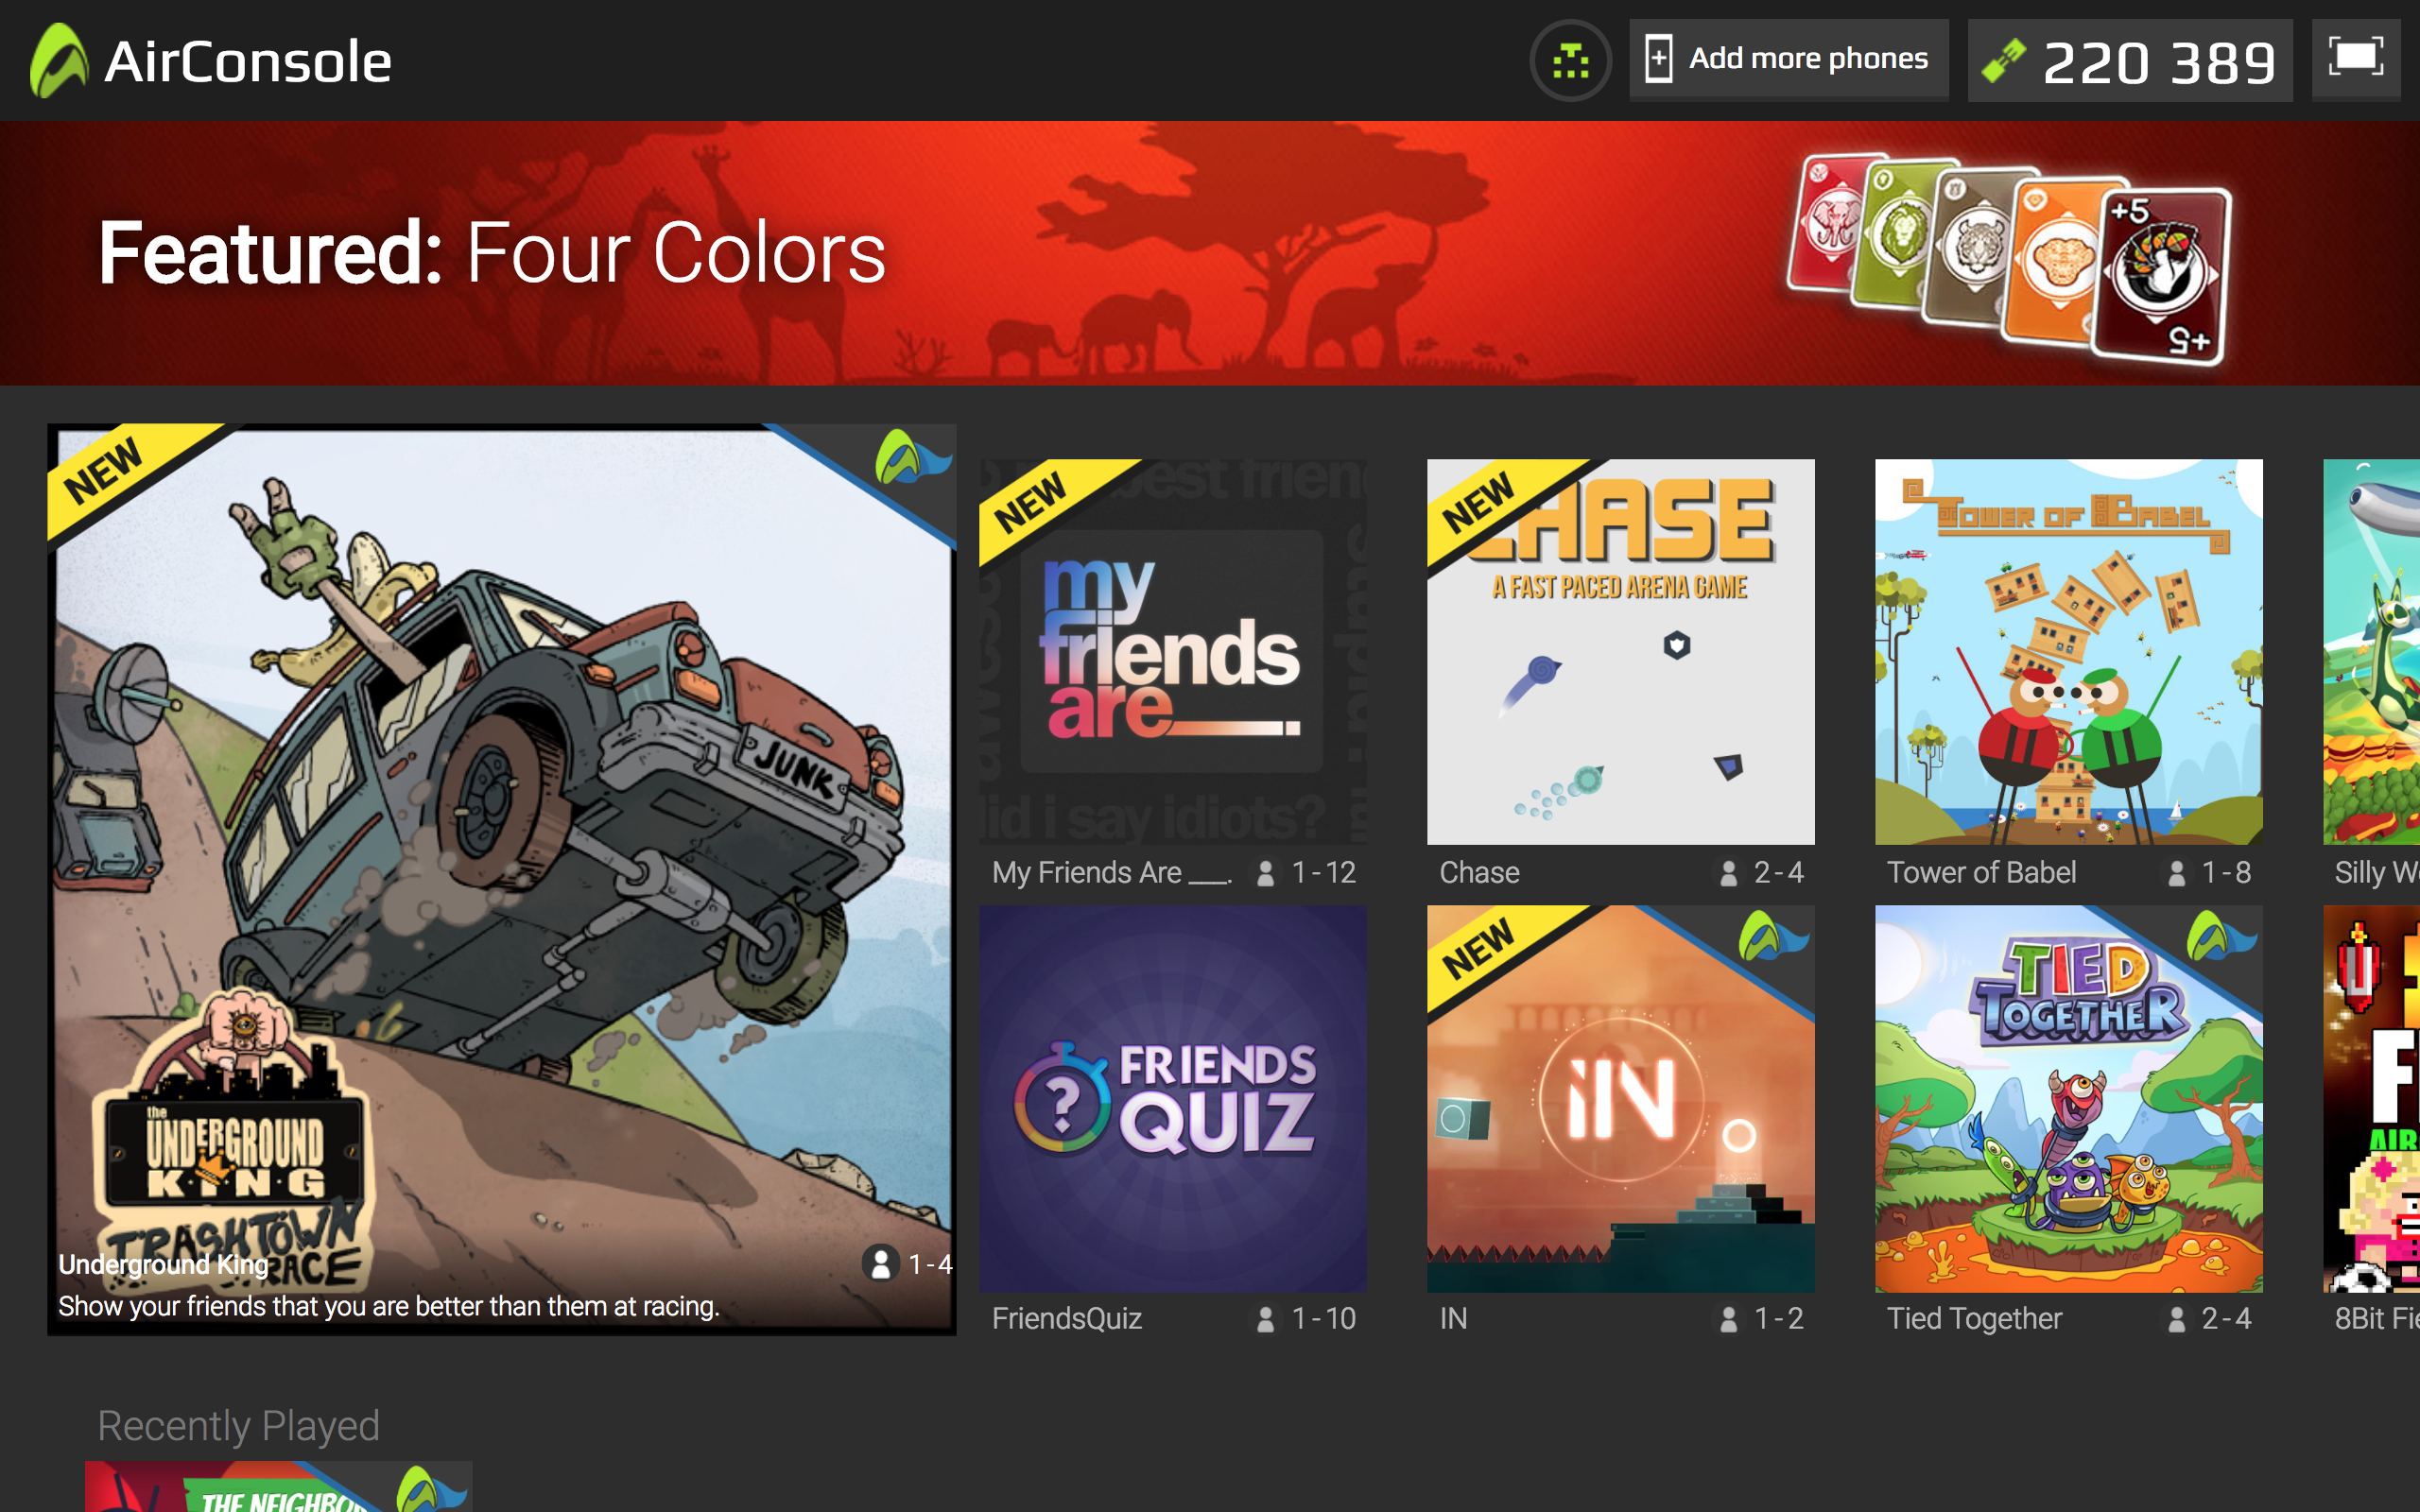
\includegraphics[scale=0.3]{Gambar/con3_play1}
	\caption{Halaman pada \textit{PC} yang menunjukan berbagai permainan yang dapat dipilih.}
	\label{fig:21_con3_play1}
\end{figure}

	\textbf{Smartphone}
	
	Halaman ini merupakan halaman utama yang pertama kali dituju oleh pengguna yang menggunakan \textit{smartphone}. Komponen halaman ini terdiri dari teks yang menunjukan nama permainan yaitu \textit{finger for life}, dan tombol \textit{join} yang digunakan untuk memulai permainan. Rancangan antarmuka halaman \textit{home} dapat dilihat pada Gambar \ref{fig:22_con3_play1}.
	
\begin{figure}[H]
	\centering
	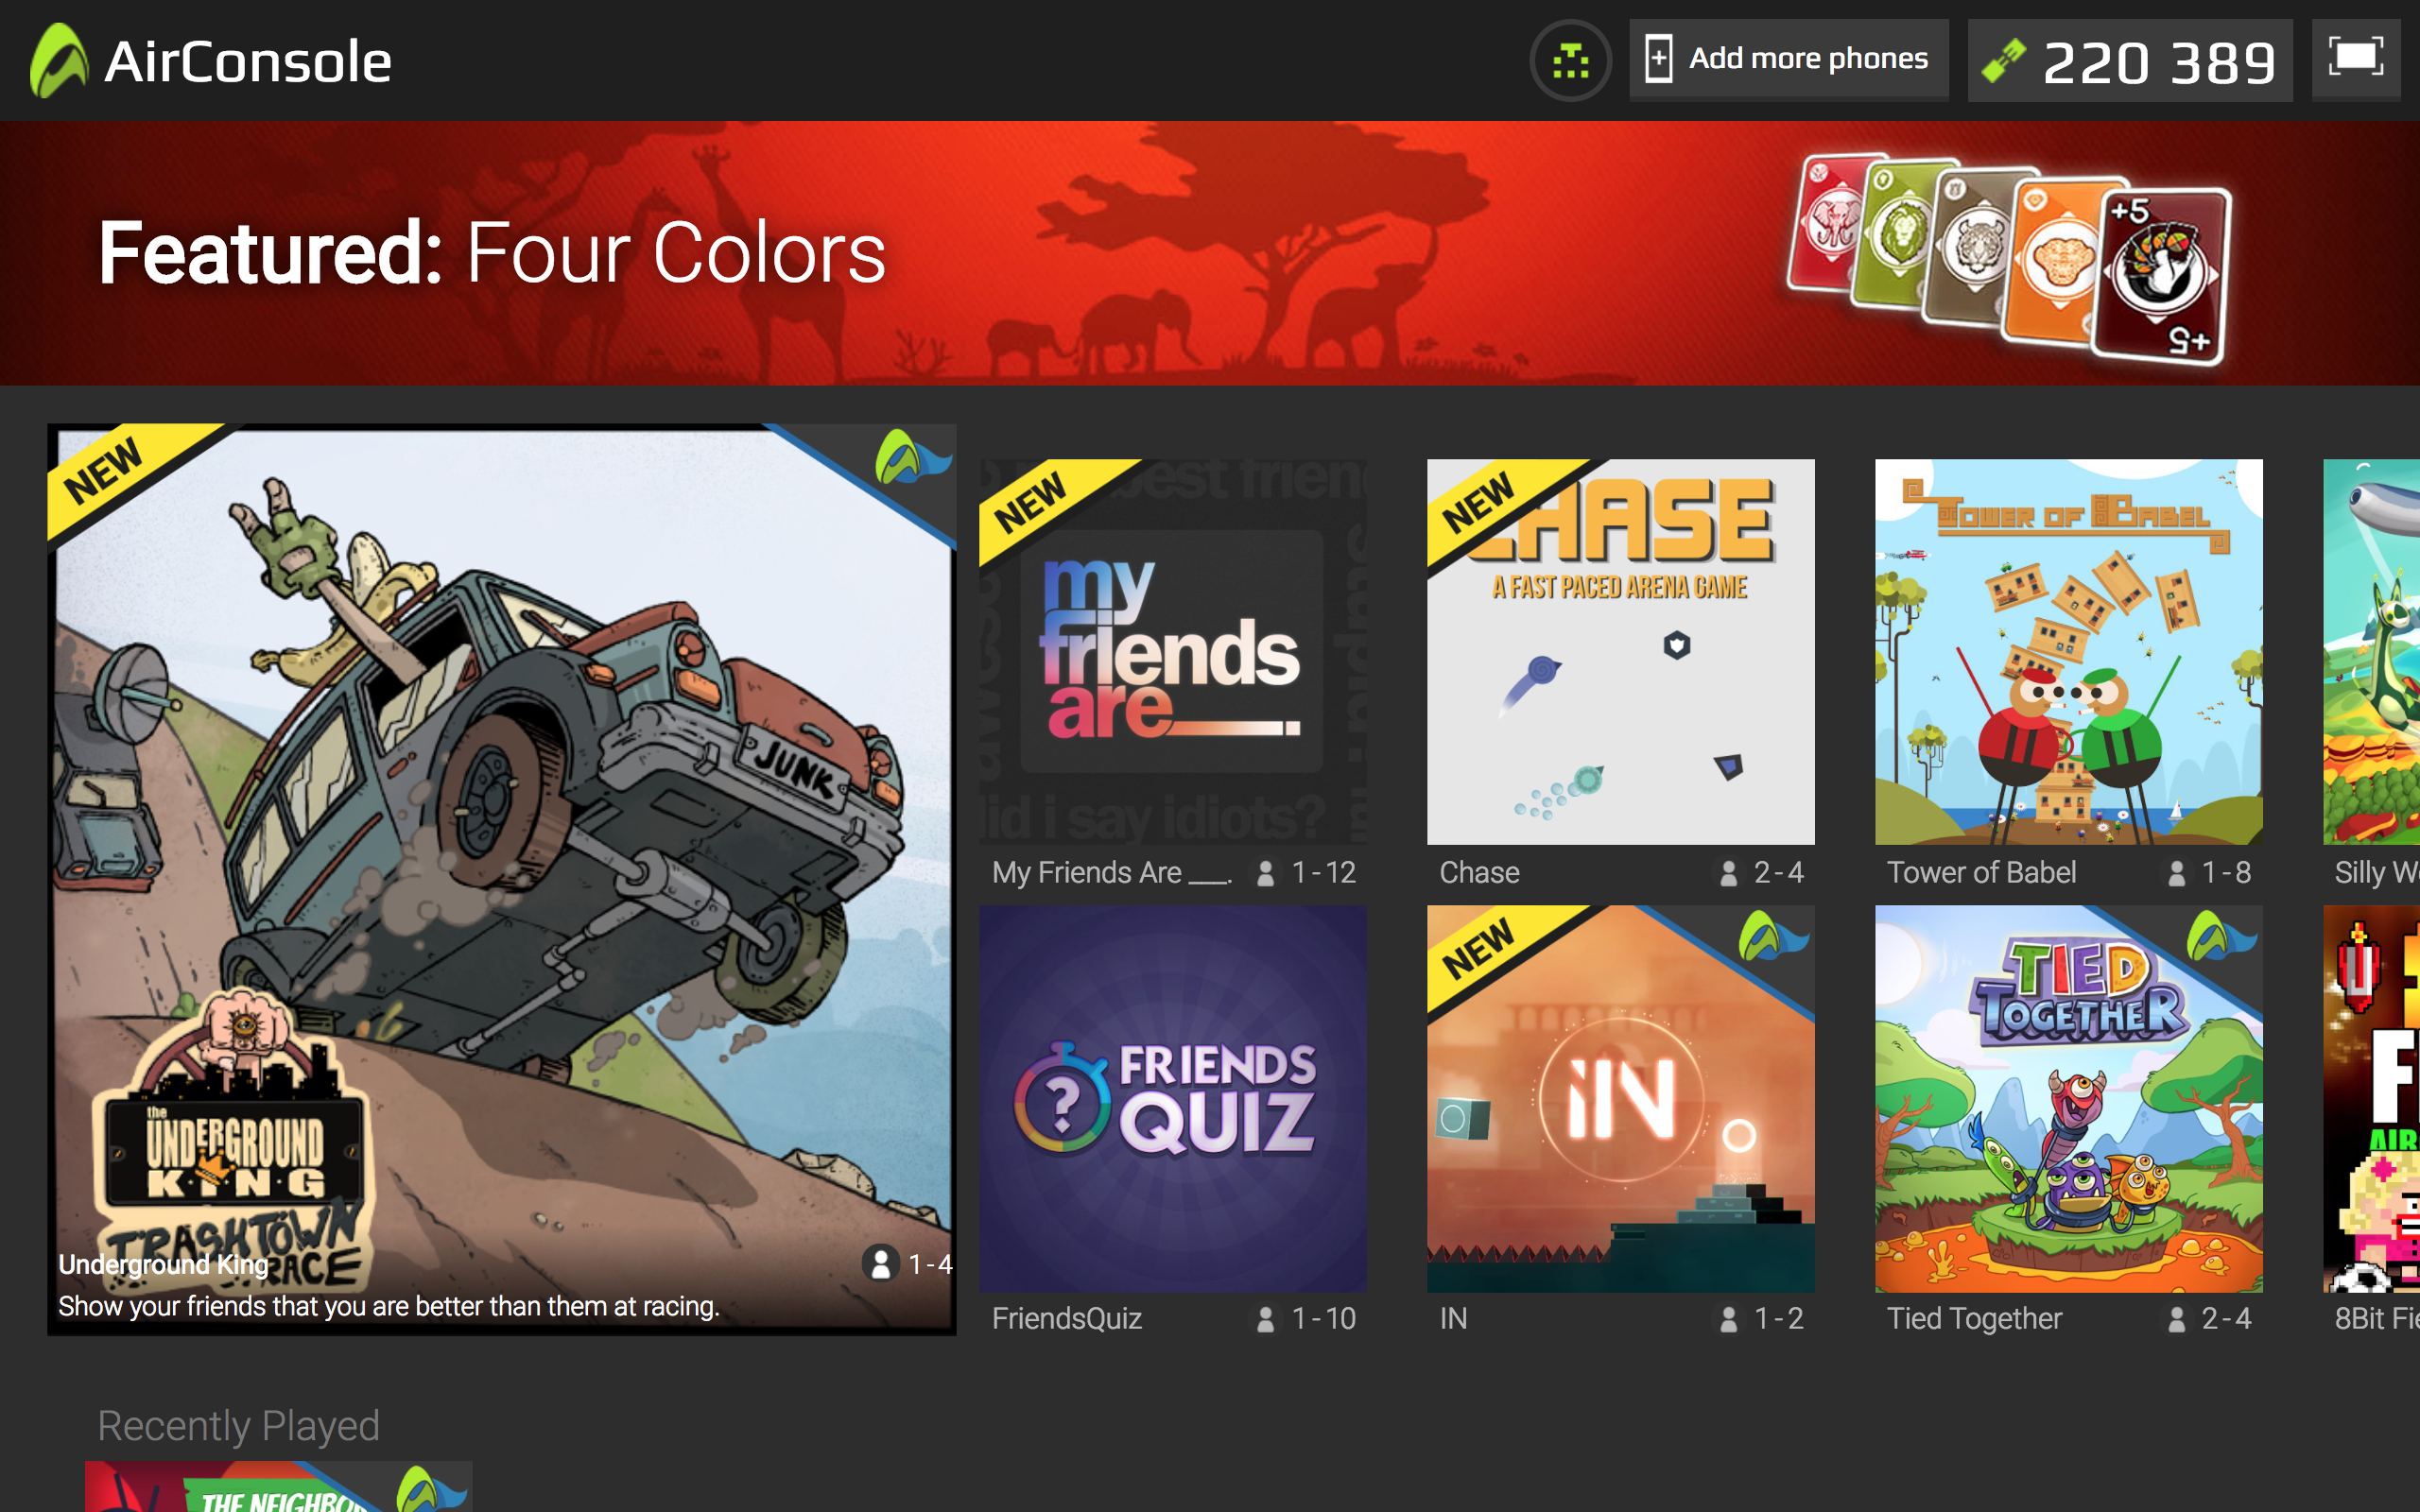
\includegraphics[scale=0.3]{Gambar/con3_play1}
	\caption{Halaman pada \textit{PC} yang menunjukan berbagai permainan yang dapat dipilih.}
	\label{fig:22_con3_play1}
\end{figure}

	\item Antarmuka halaman \textit{sync}
	
	\textbf{PC}
	
	Halaman ini menampilkan suatu perintah yang dapat dilakukan oleh pengguna apabila akan bergabung dalam permainan. Halaman ini pun menyediakan suatu kode untuk para pemain dimana kode tersebut akan berfungsi sebagai suatu \textit{room} bagi para pemain. Pada halaman ini akan dilakukan proses sinkronisasi untuk para pengguna, apakah berhasil bergabung dalam permainan atau tidak. Apabila berhasil, maka akan muncul suatu teks yang menunjukan suatu pemain telah berhasil bergabung. Apabila tidak, maka tidak akan menampilkan apapun dan halaman tidak akan menuju ke halaman selanjutnya sebelum ada dua pemain yang berhasil bergabung. Rancangan antarmuka halaman \textit{sync} pada \textit{PC} dapat dilihat pada Gambar \ref{fig:23_con3_play1}.
	
\begin{figure}[H]
	\centering
	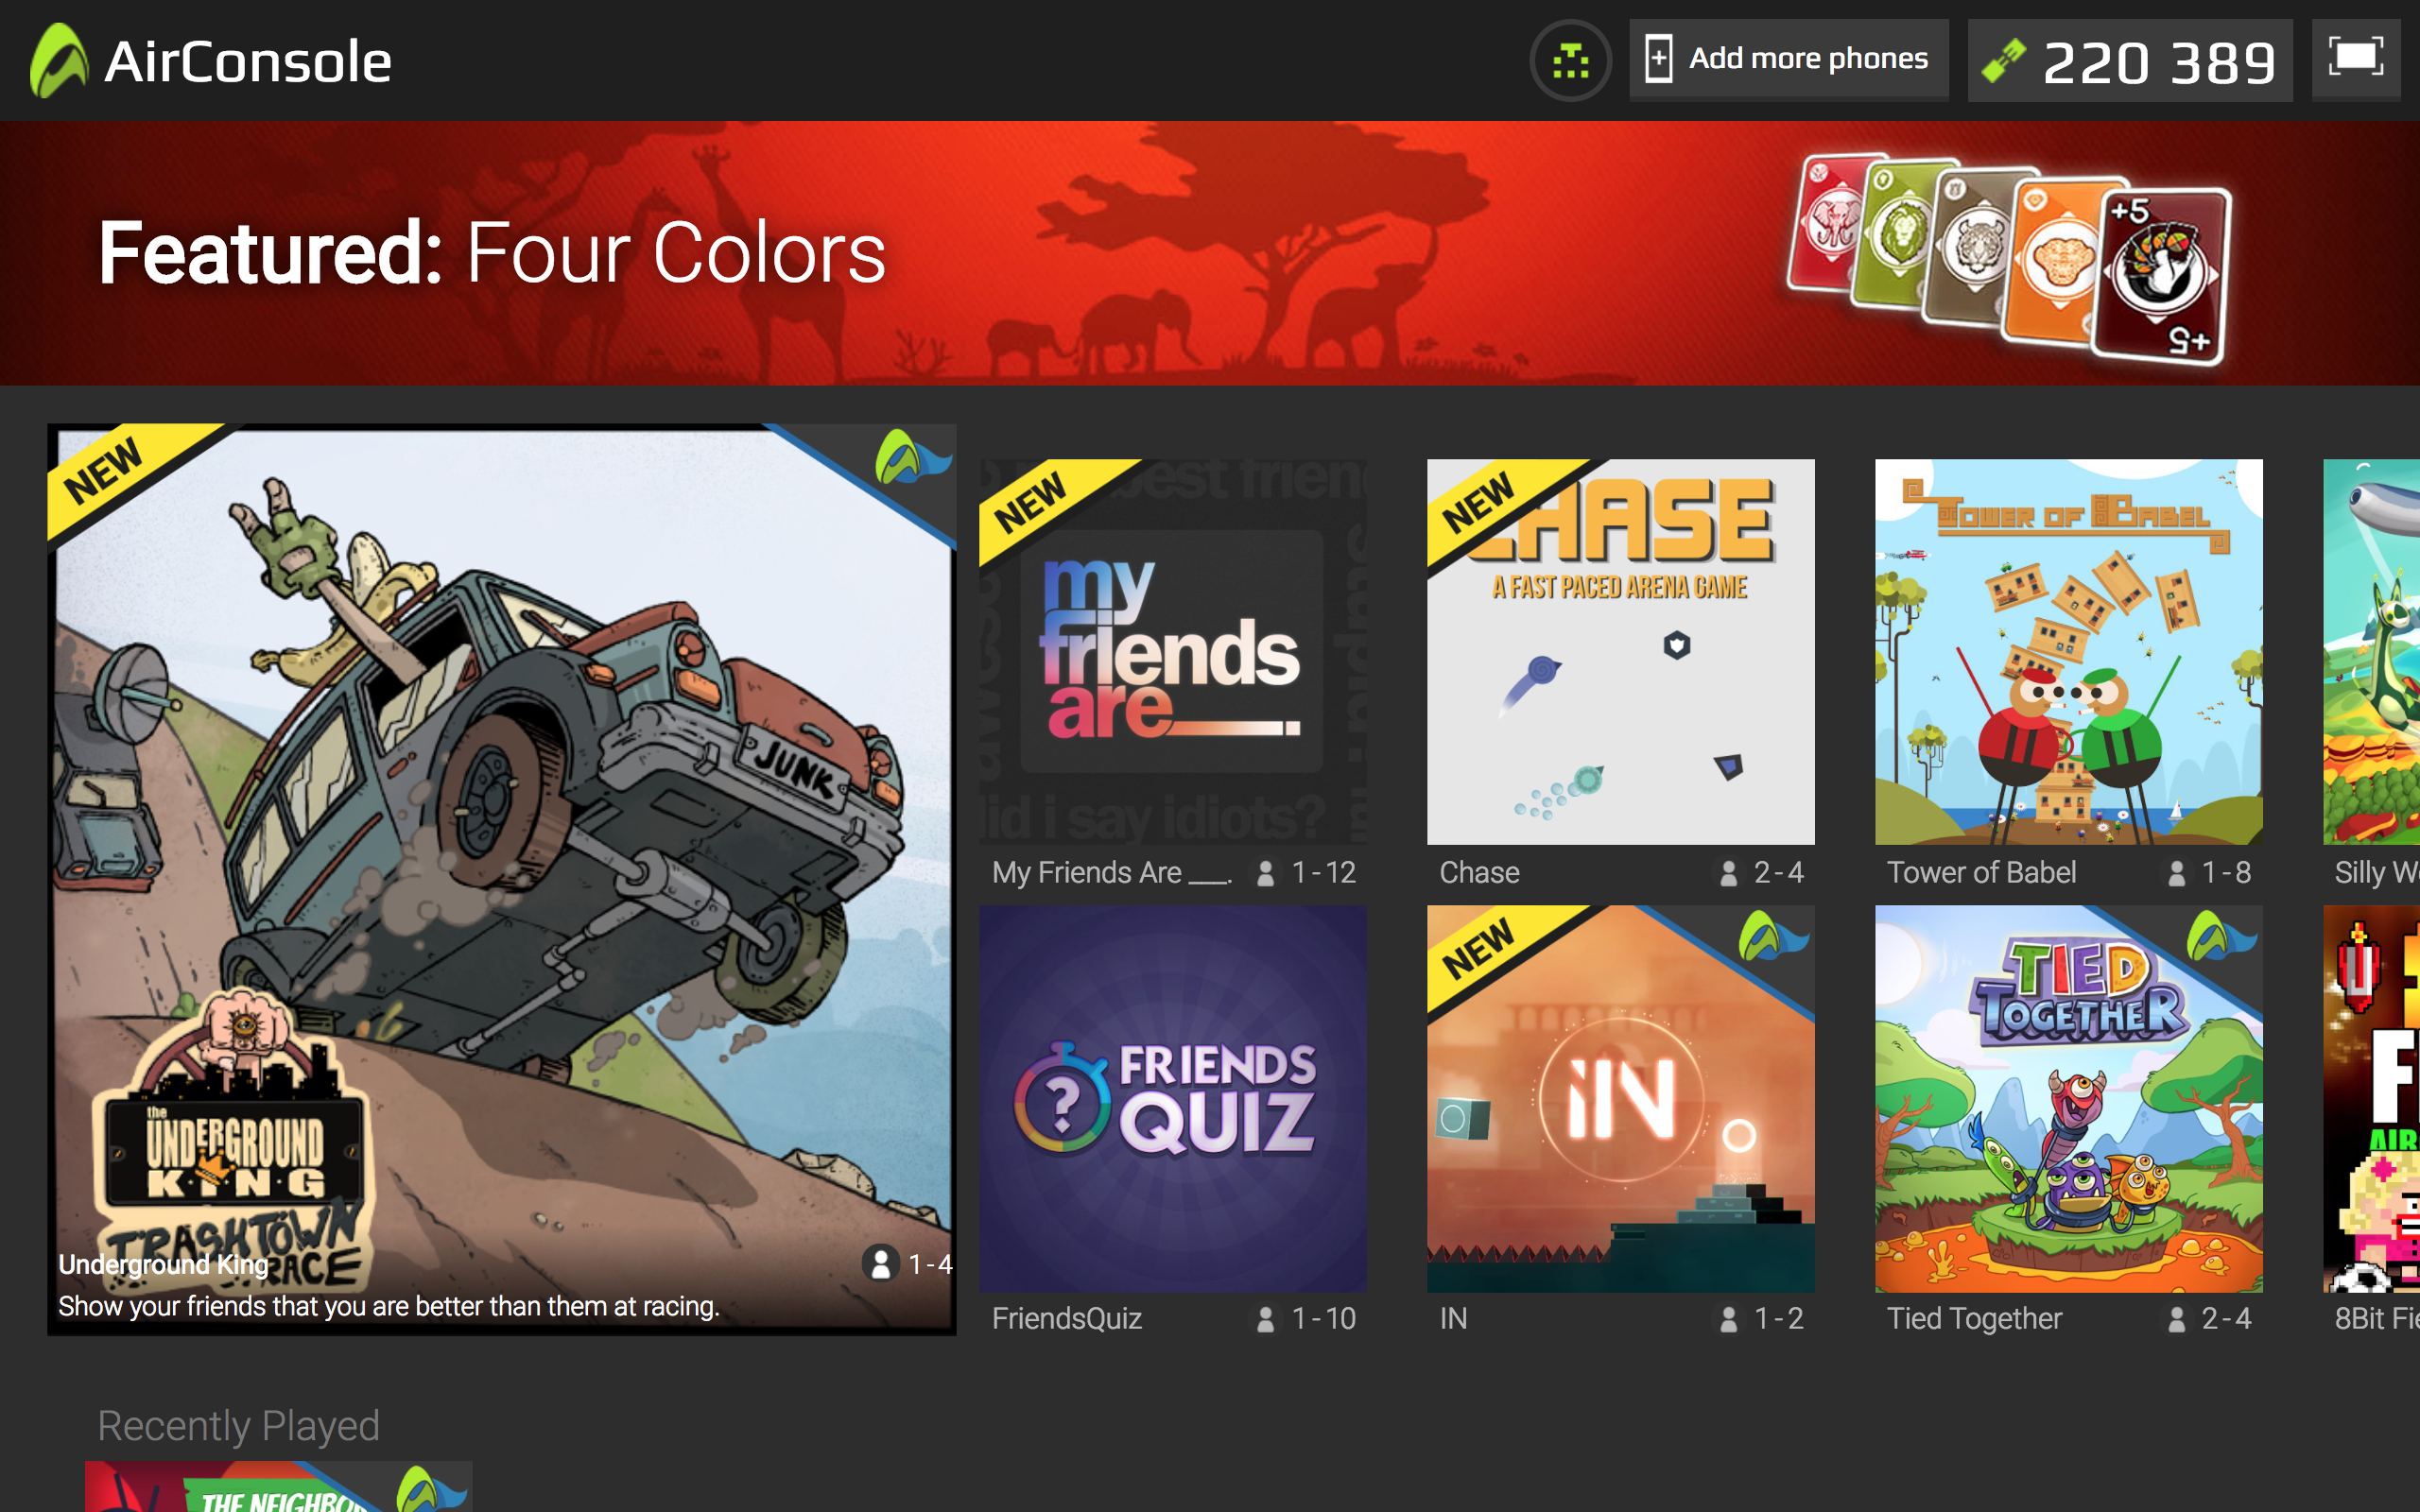
\includegraphics[scale=0.3]{Gambar/con3_play1}
	\caption{Halaman pada \textit{PC} yang menunjukan berbagai permainan yang dapat dipilih.}
	\label{fig:23_con3_play1}
\end{figure}

	\textbf{Smartphone}
	
	Halaman ini berfungsi untuk melakukan \textit{request} untuk bergabung dalam permainan. Komponen halaman ini terdiri dari kolom kode, dan tombol \textit{send}. Rancangan antarmuka halaman \textit{sync} pada \textit{smartphone} dapat dilihat pada Gambar \ref{fig:24_con3_play1}.
	
\begin{figure}[H]
	\centering
	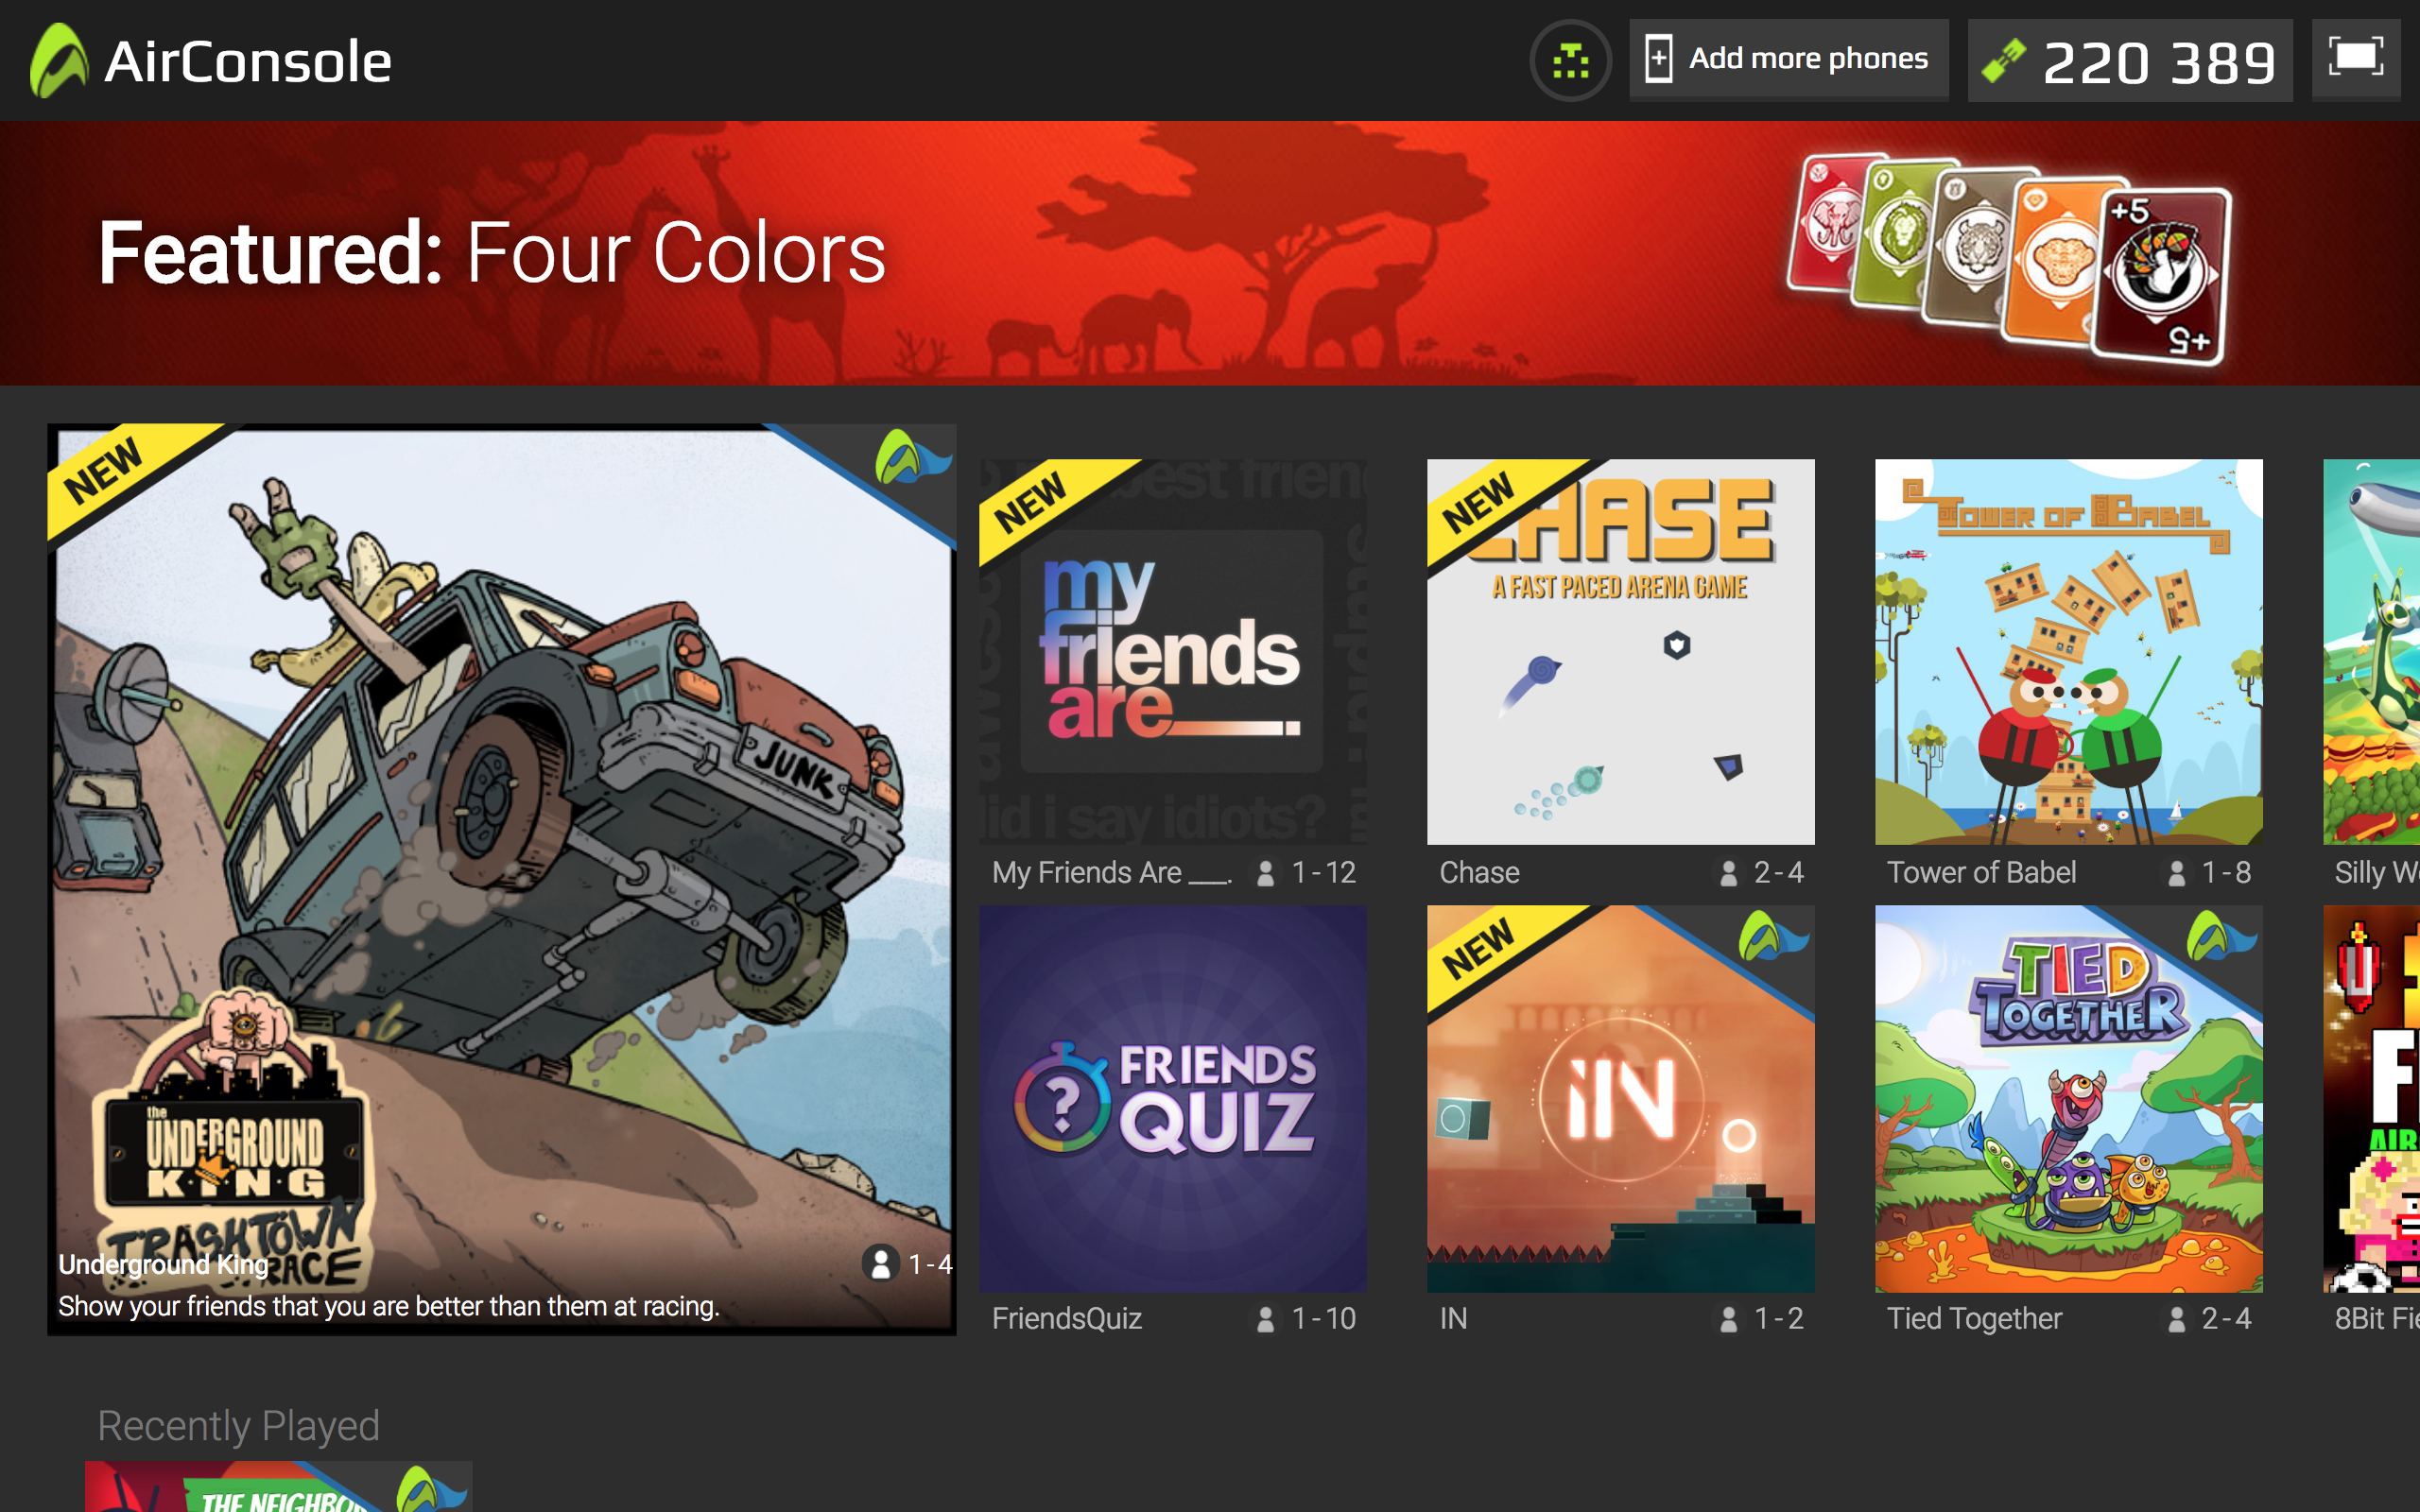
\includegraphics[scale=0.3]{Gambar/con3_play1}
	\caption{Halaman pada \textit{PC} yang menunjukan berbagai permainan yang dapat dipilih.}
	\label{fig:24_con3_play1}
\end{figure}

\item Antarmuka halaman \textit{character}

	\textbf{PC}
	
	Halaman ini akan menampilkan karakter yang telah dipilih oleh pemain. Apabila karakter belum memilih karakter yang akan dimainkan, maka halaman ini belum menampilkan apapun. Rancangan antarmuka halaman \textit{character} pada \textit{PC} dapat dilihat pada Gambar \ref{fig:25_con3_play1}.
	
\begin{figure}[H]
	\centering
	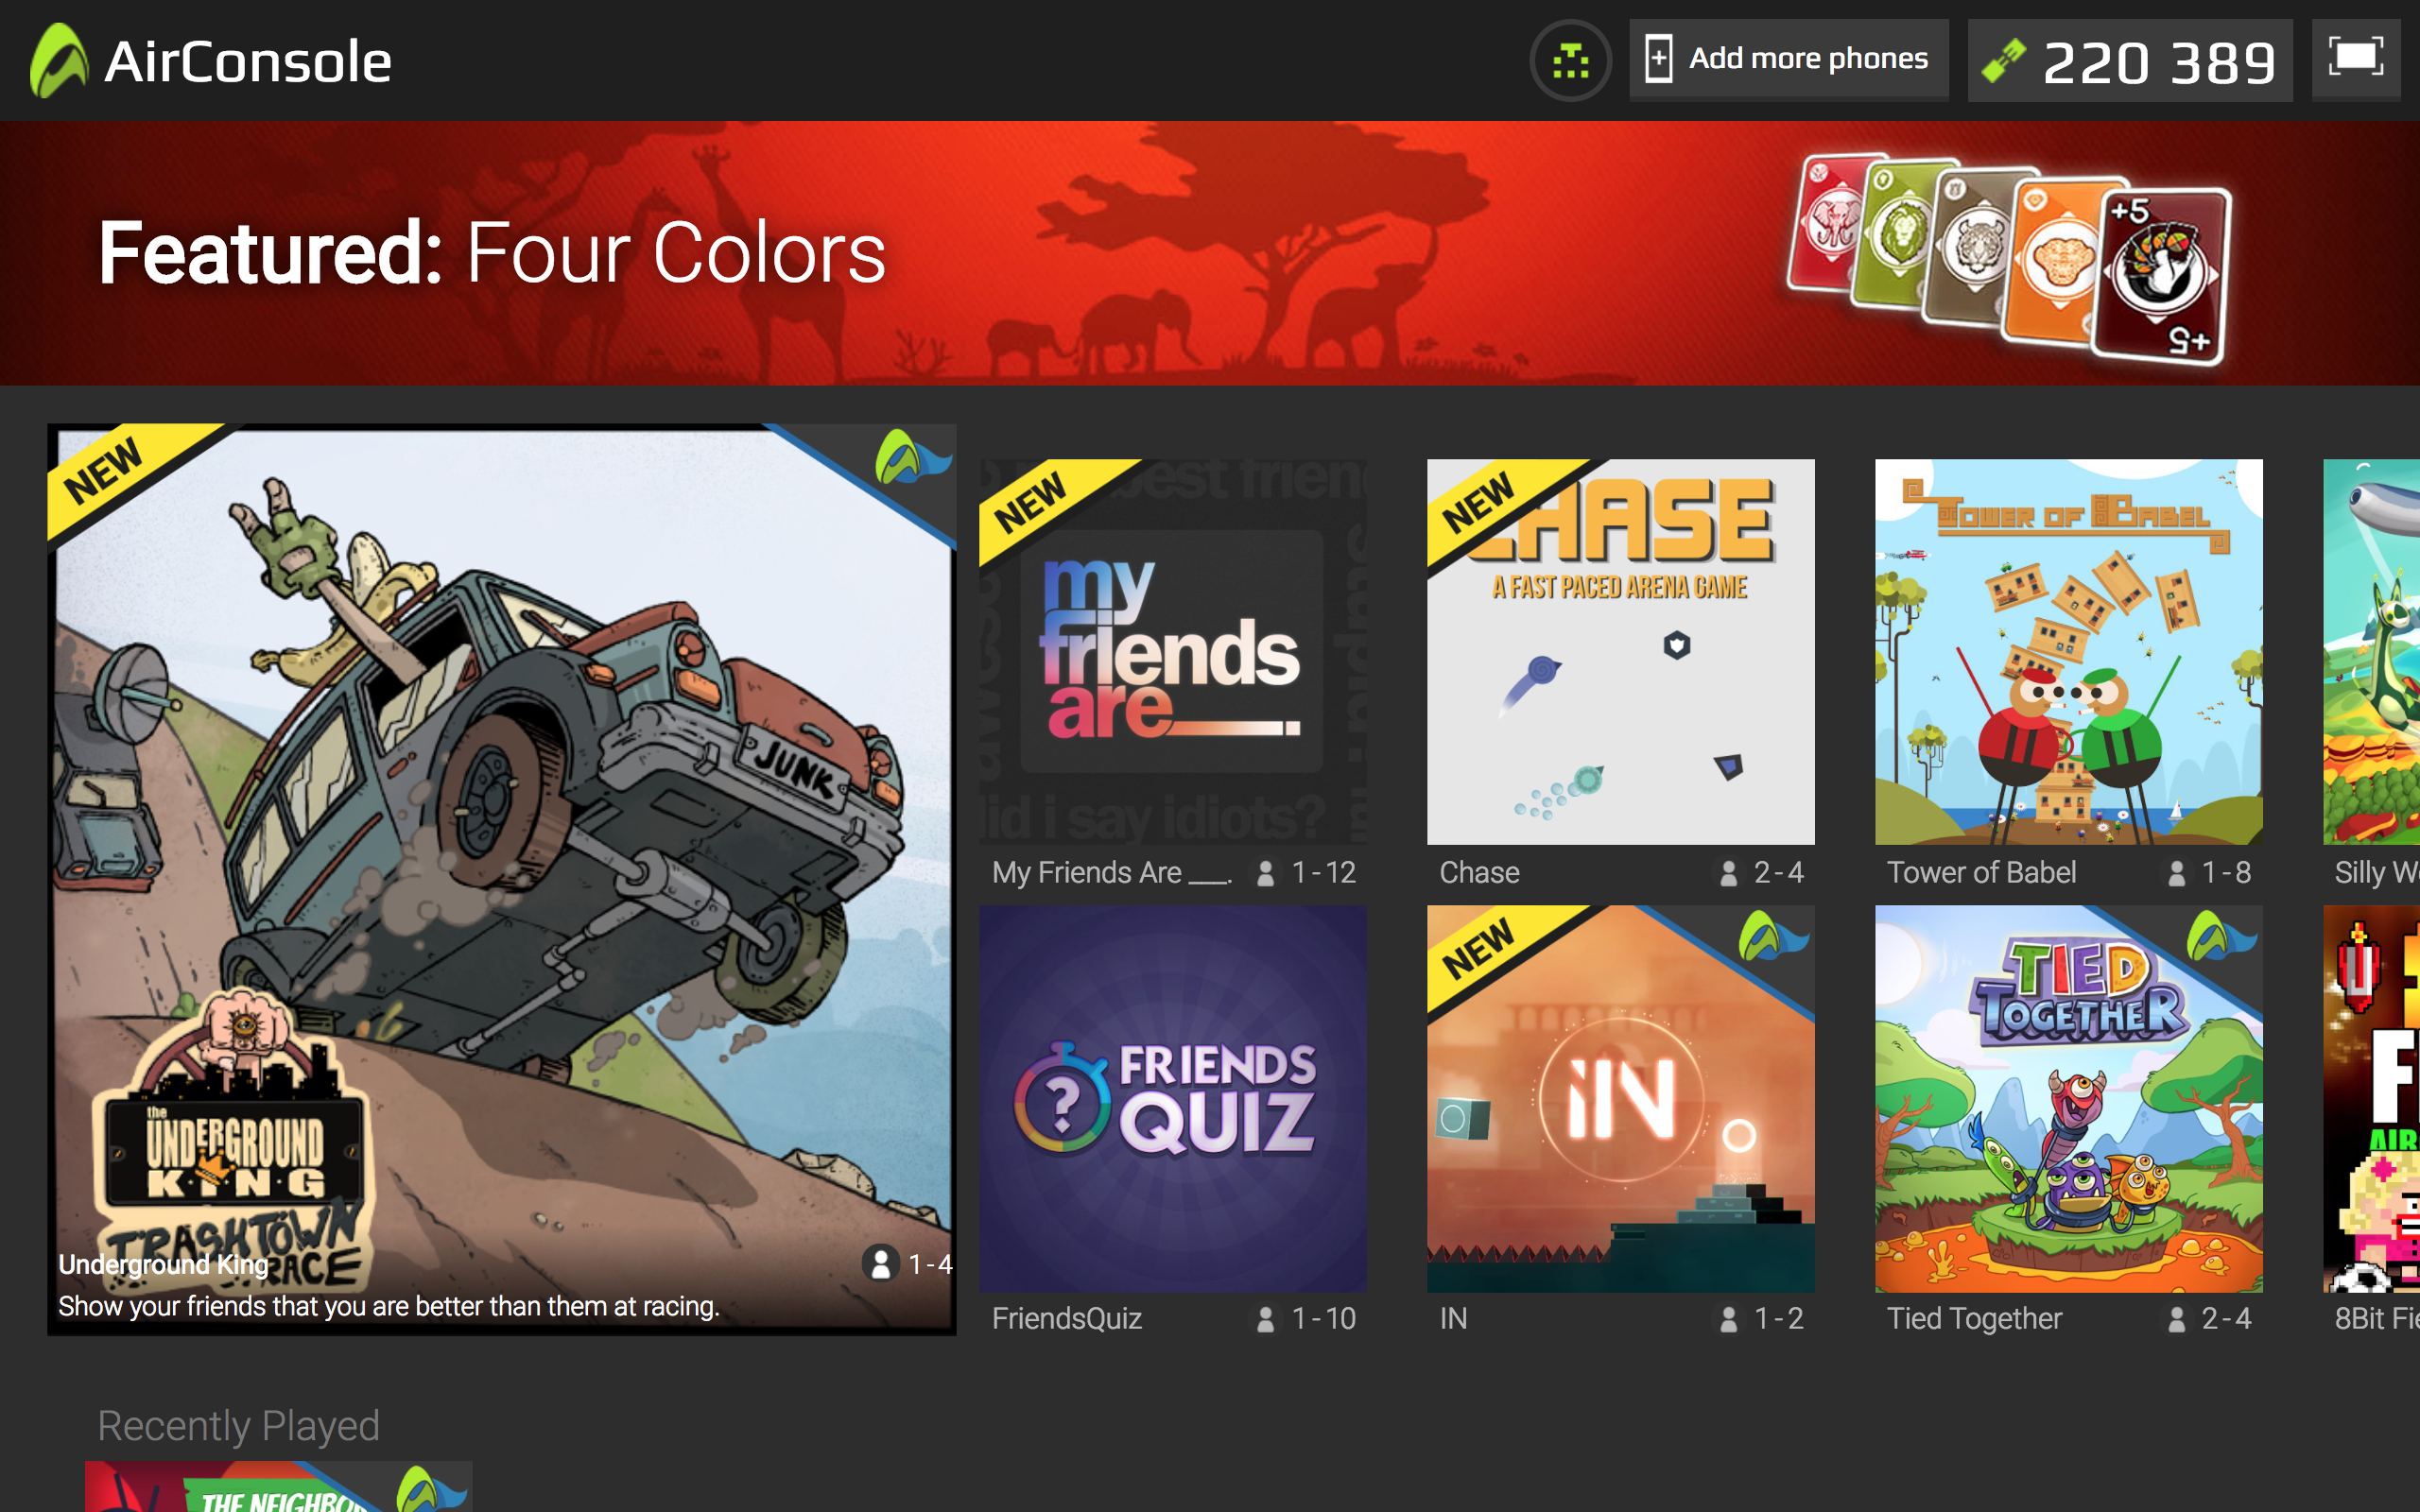
\includegraphics[scale=0.3]{Gambar/con3_play1}
	\caption{Halaman pada \textit{PC} yang menunjukan berbagai permainan yang dapat dipilih.}
	\label{fig:25_con3_play1}
\end{figure}


	\textbf{Smartphone}
	
	Halaman ini akan menampilkan daftar karakter yang dapat dimainkan oleh pemain. Komponen halaman ini terdiri dari daftar karakter, dan tombol \textit{choose}. Rancangan antarmuka halaman \textit{character} pada \textit{smartphone} dapat dilihat pada Gambar \ref{fig:26_con3_play1}.
	
\begin{figure}[H]
	\centering
	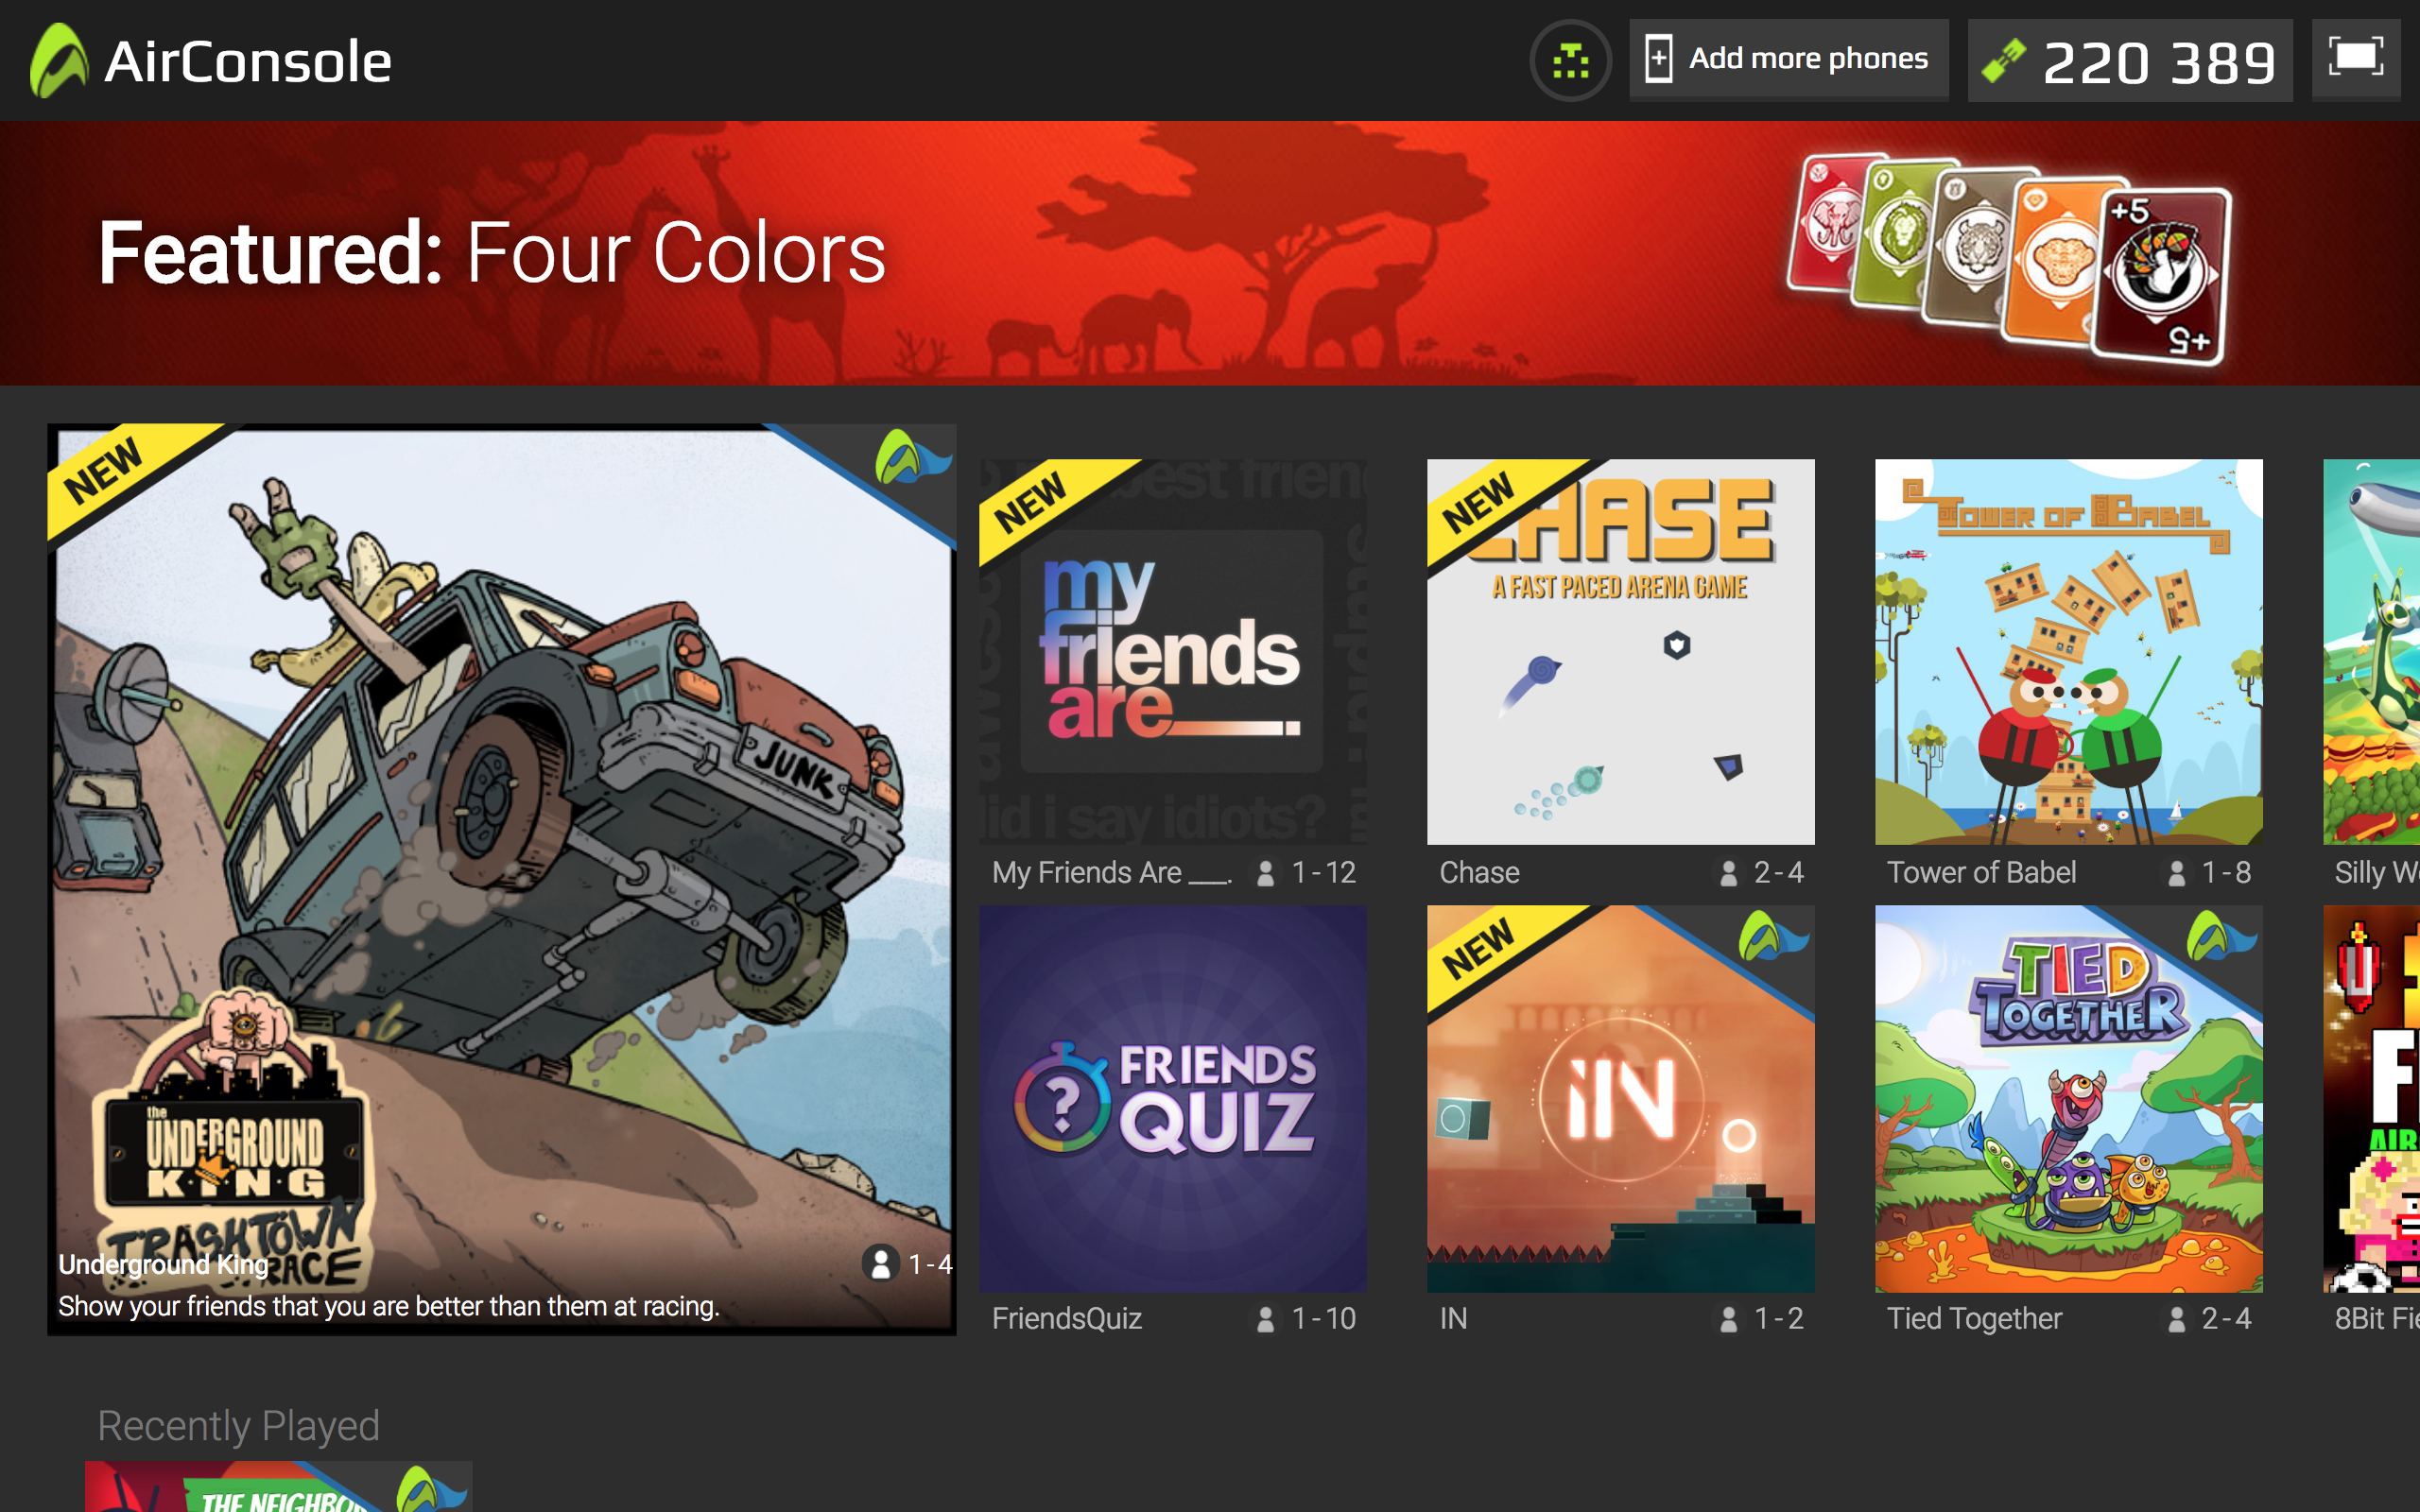
\includegraphics[scale=0.3]{Gambar/con3_play1}
	\caption{Halaman pada \textit{PC} yang menunjukan berbagai permainan yang dapat dipilih.}
	\label{fig:26_con3_play1}
\end{figure}

\item Antarmuka halaman \textit{gameplay}

	\textbf{PC}
	
	Halaman ini menampilkan arena permainan untuk para pemain. Komponen halaman ini terdiri dari suatu gambar lintasan lari, dan karakter yang telah dipilih pada halaman sebelumnya. Rancangan antarmuka halaman \textit{gameplay} pada \textit{PC} dapat dilihat pada Gambar \ref{fig:27_con3_play1}.
	
\begin{figure}[H]
	\centering
	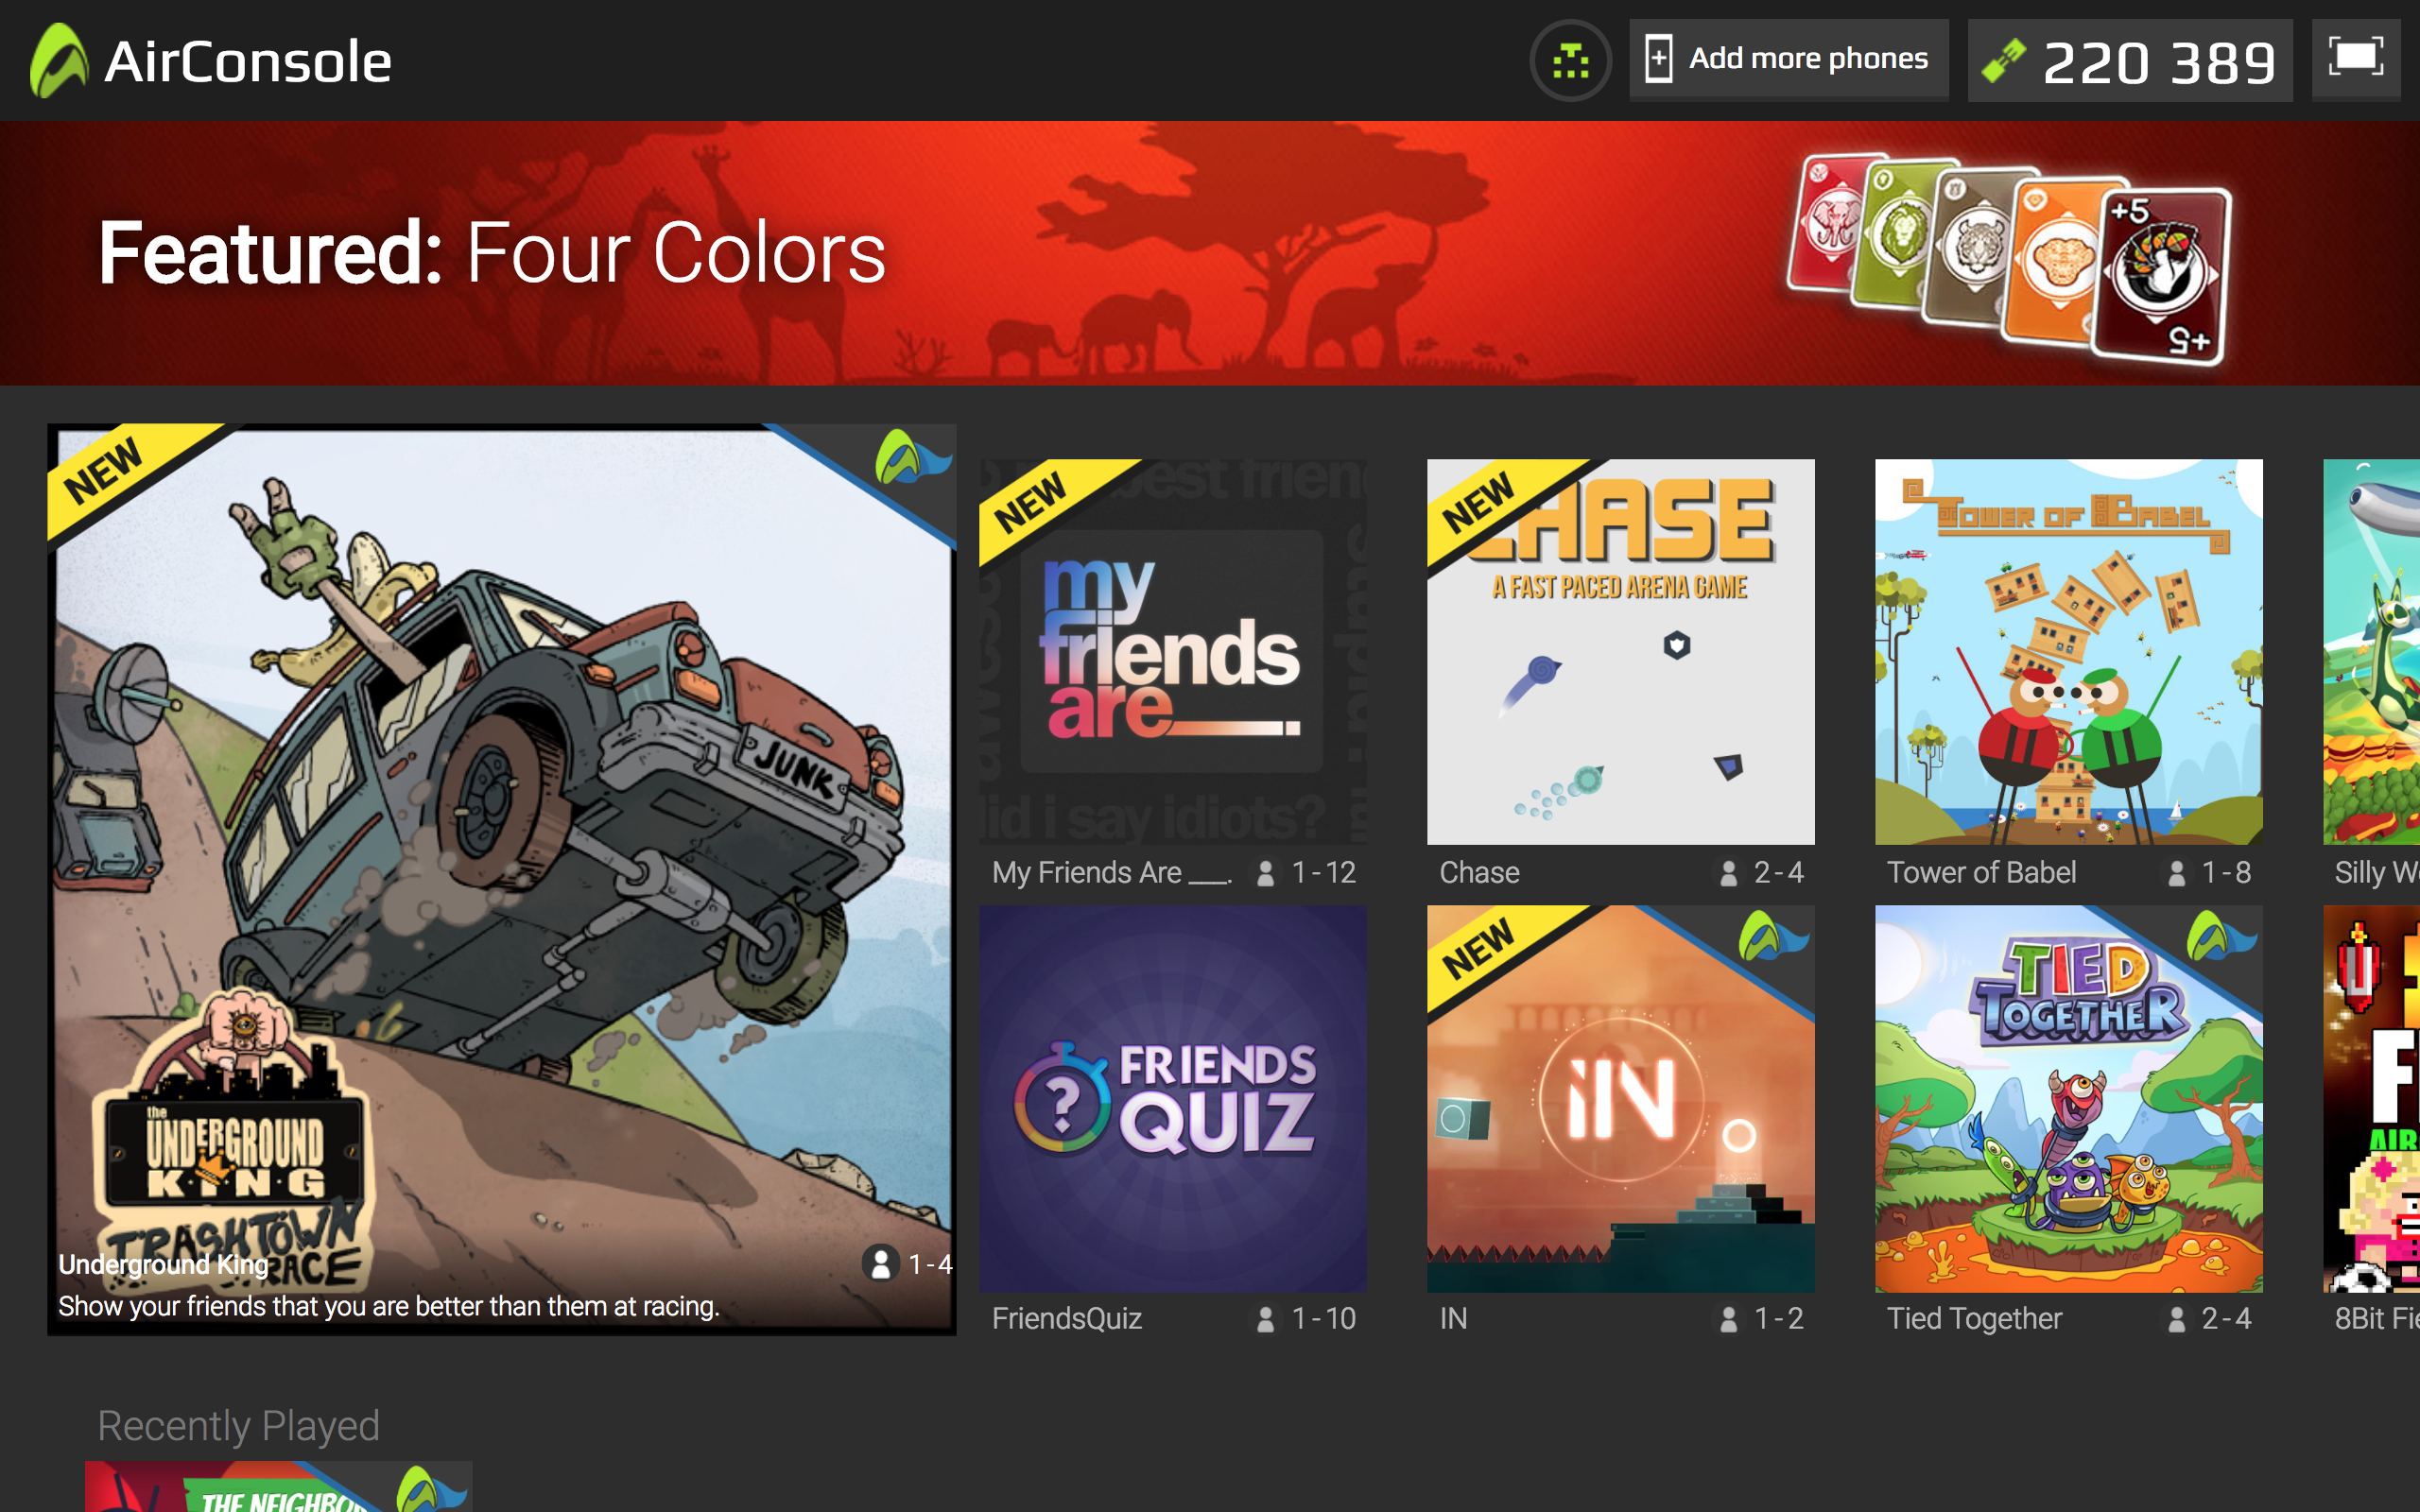
\includegraphics[scale=0.3]{Gambar/con3_play1}
	\caption{Halaman pada \textit{PC} yang menunjukan berbagai permainan yang dapat dipilih.}
	\label{fig:27_con3_play1}
\end{figure}

	\textbf{Smartphone}
	
	Halaman ini berfungsi sebagai \textit{controller} untuk para pemain. Komponen halaman ini terdiri dari dua buah gambar telapak kaki yang berfungsi sebagai tombol. Pemain dapat menekan tombol berulang kali untuk menggerakan karakter yang ada pada halaman \textit{gameplay} di \textit{PC}. Rancangan antarmuka halaman \textit{gameplay} pada \textit{smartphone} dapat dilihat pada Gambar \ref{fig:28_con3_play1}.
	
\begin{figure}[H]
	\centering
	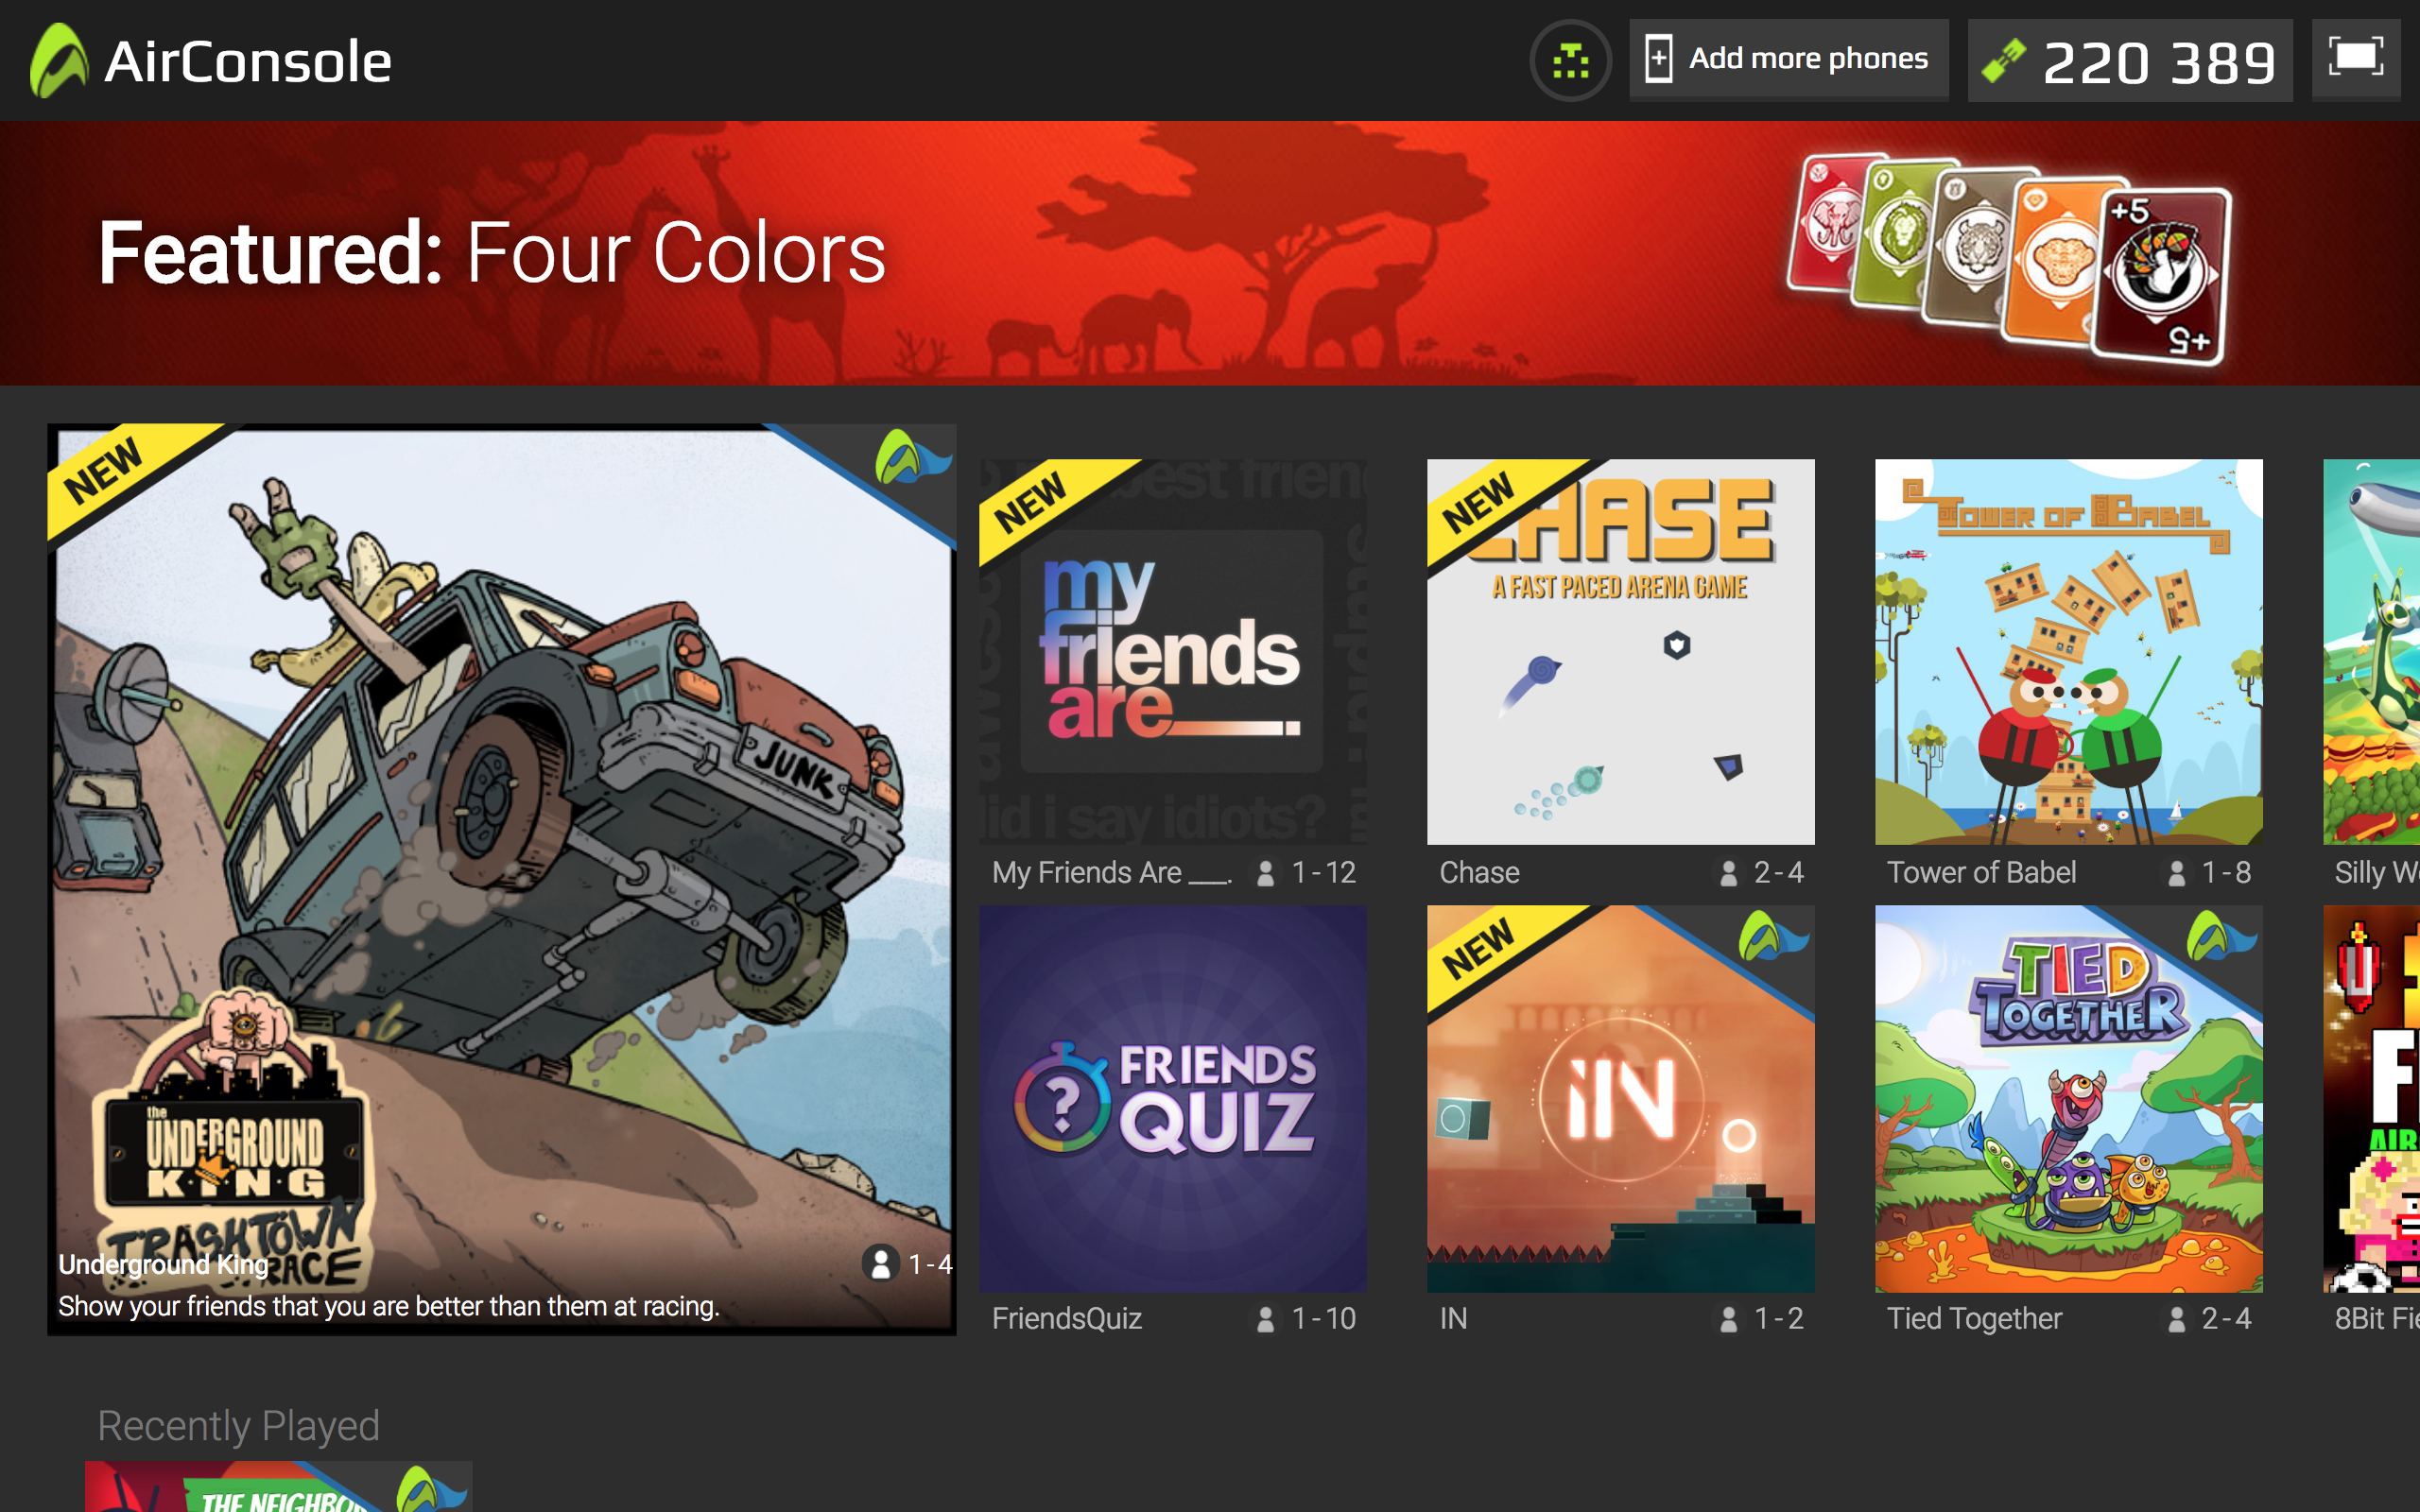
\includegraphics[scale=0.3]{Gambar/con3_play1}
	\caption{Halaman pada \textit{PC} yang menunjukan berbagai permainan yang dapat dipilih.}
	\label{fig:28_con3_play1}
\end{figure}

\item Antarmuka halaman \textit{gameover}

	\textbf{PC}
	
	Halaman ini menampilkan para pemenang yang telah berhasil menyelesaikan permainan. Setelah pemain selesai bermain, pemain dapat menekan tombol \textit{back} untuk kembali ke halaman utama dan mengakhiri permainan. Rancangan antarmuka halaman \textit{gameover} pada \textit{PC} dapat dilihat pada Gambar \ref{fig:29_con3_play1}.
	
\begin{figure}[H]
	\centering
	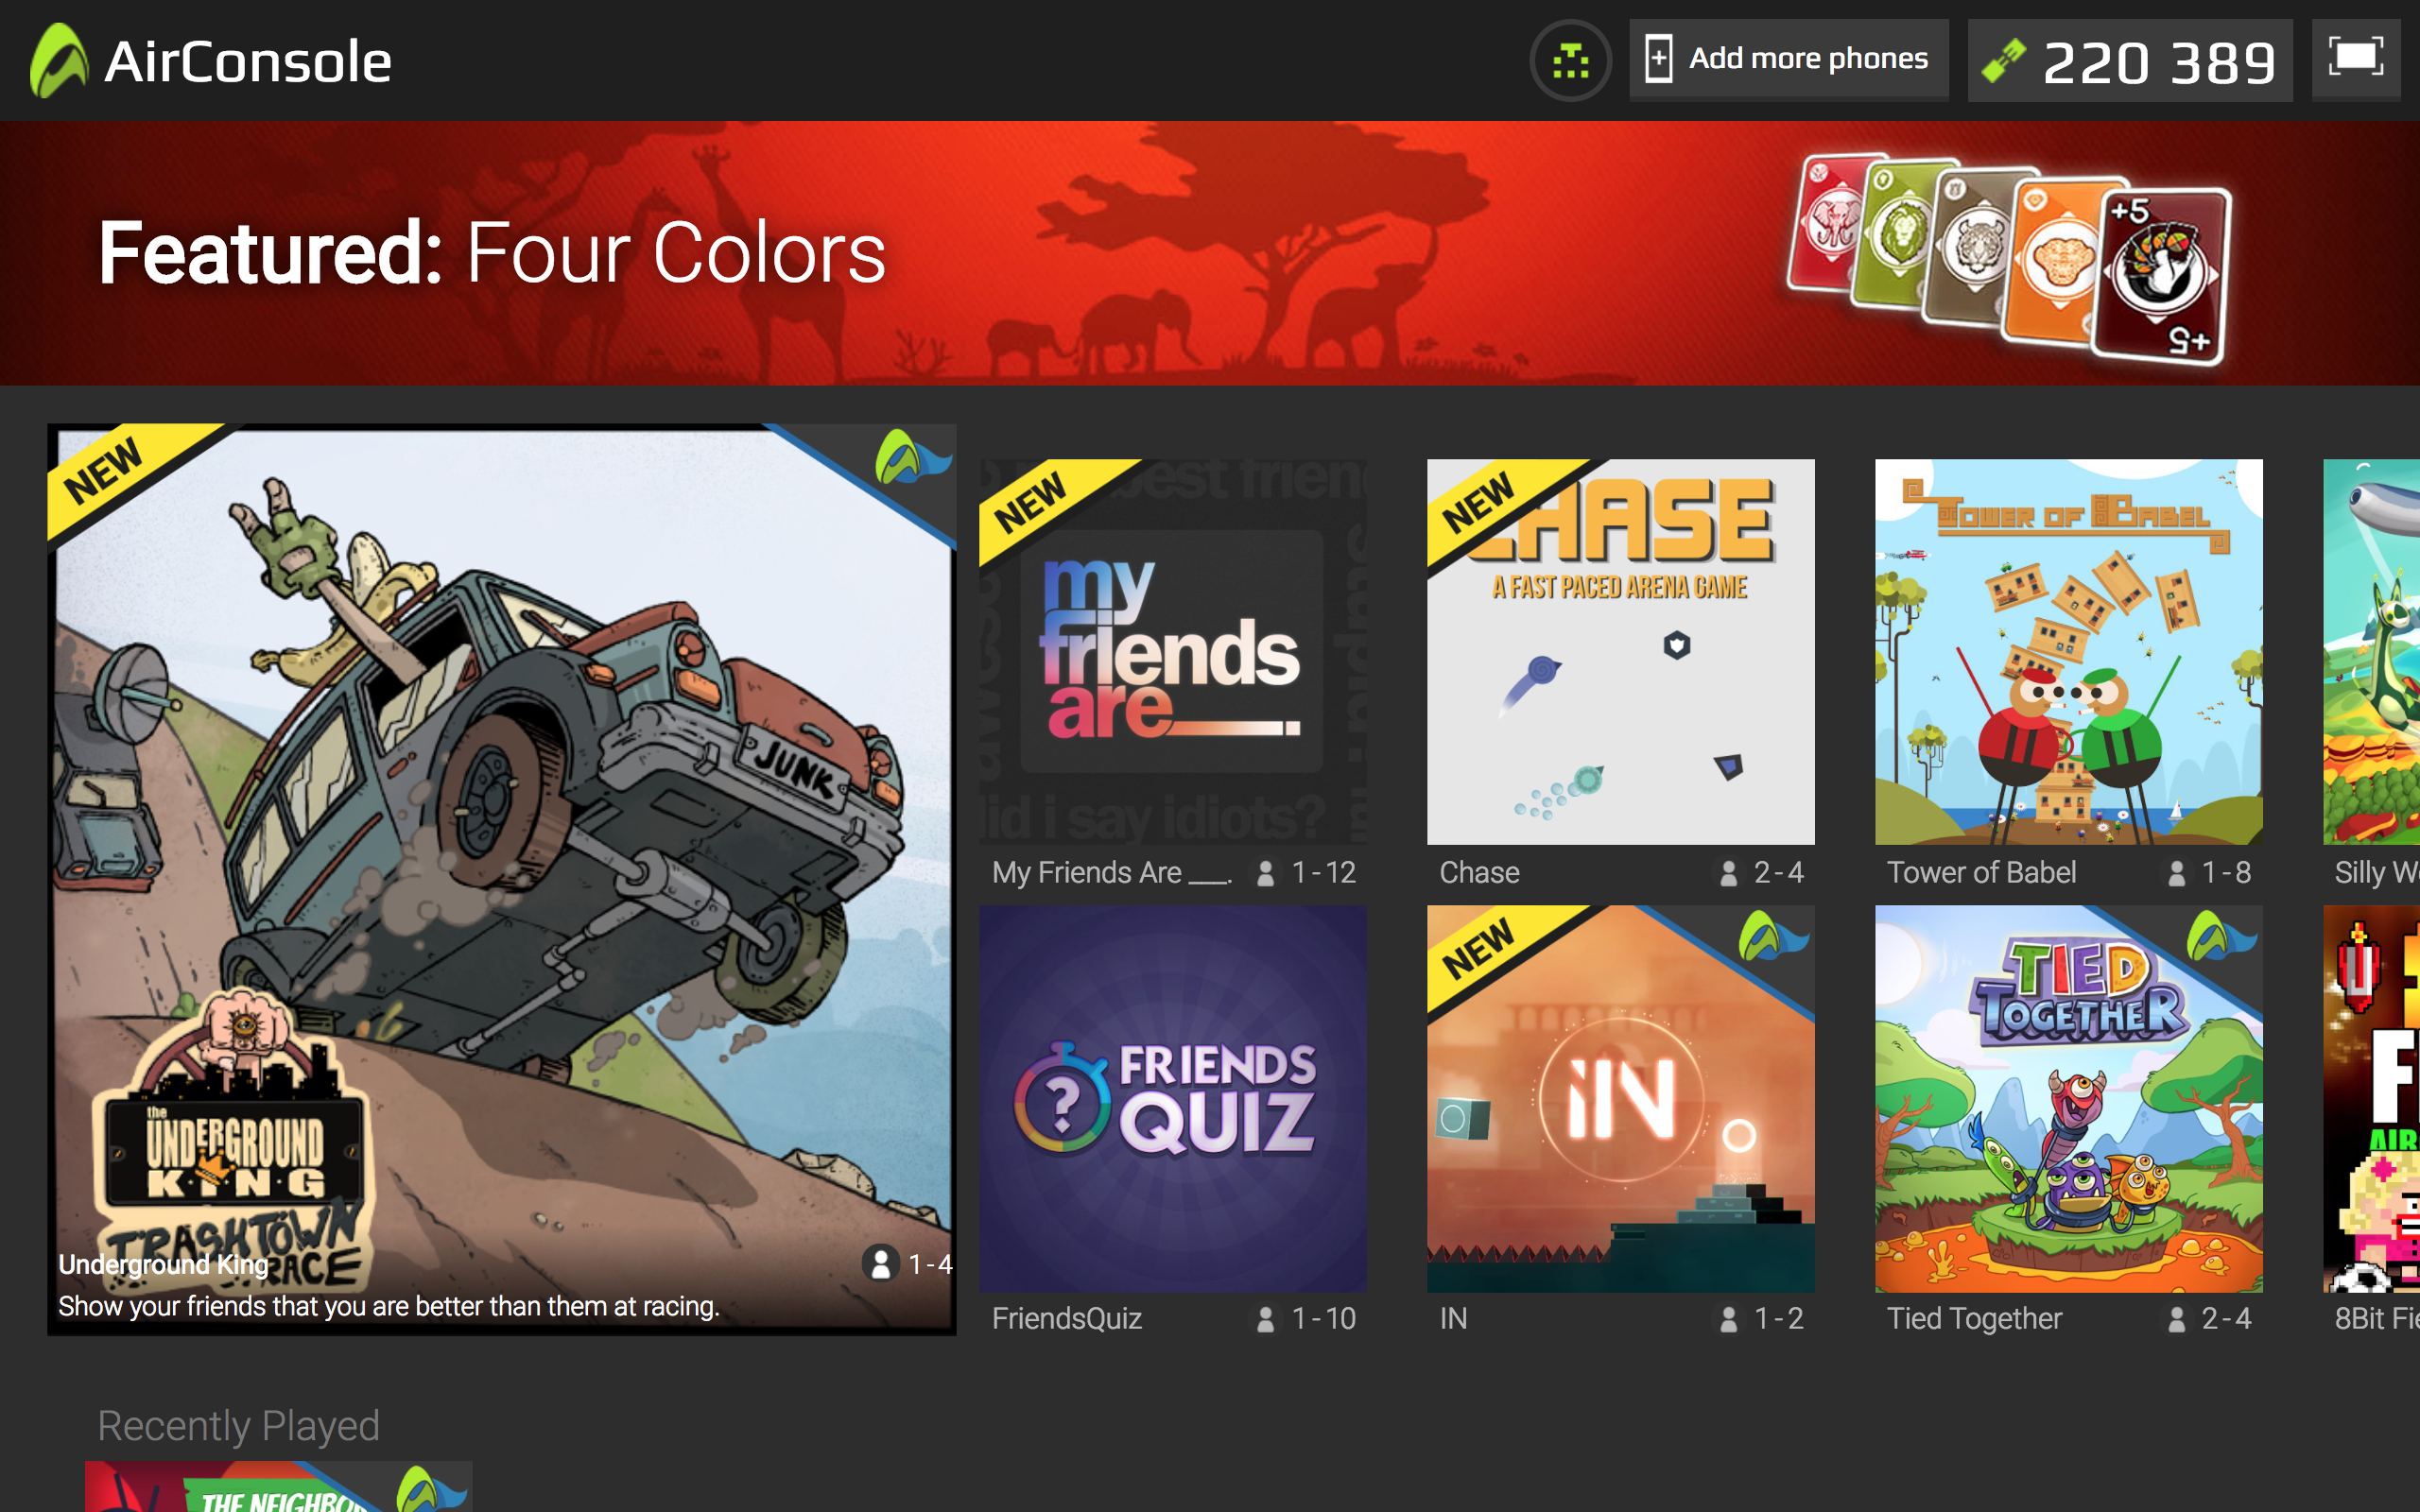
\includegraphics[scale=0.3]{Gambar/con3_play1}
	\caption{Halaman pada \textit{PC} yang menunjukan berbagai permainan yang dapat dipilih.}
	\label{fig:29_con3_play1}
\end{figure}

	\textbf{Smartphone}
	
	Halaman ini menampilkan teks yang menandakan bahwa permainan telah selesai. Rancangan antarmuka halaman \textit{gameover} pada \textit{smartphone} dapat dilihat pada Gambar \ref{fig:30_con3_play1}.
	
\begin{figure}[H]
	\centering
	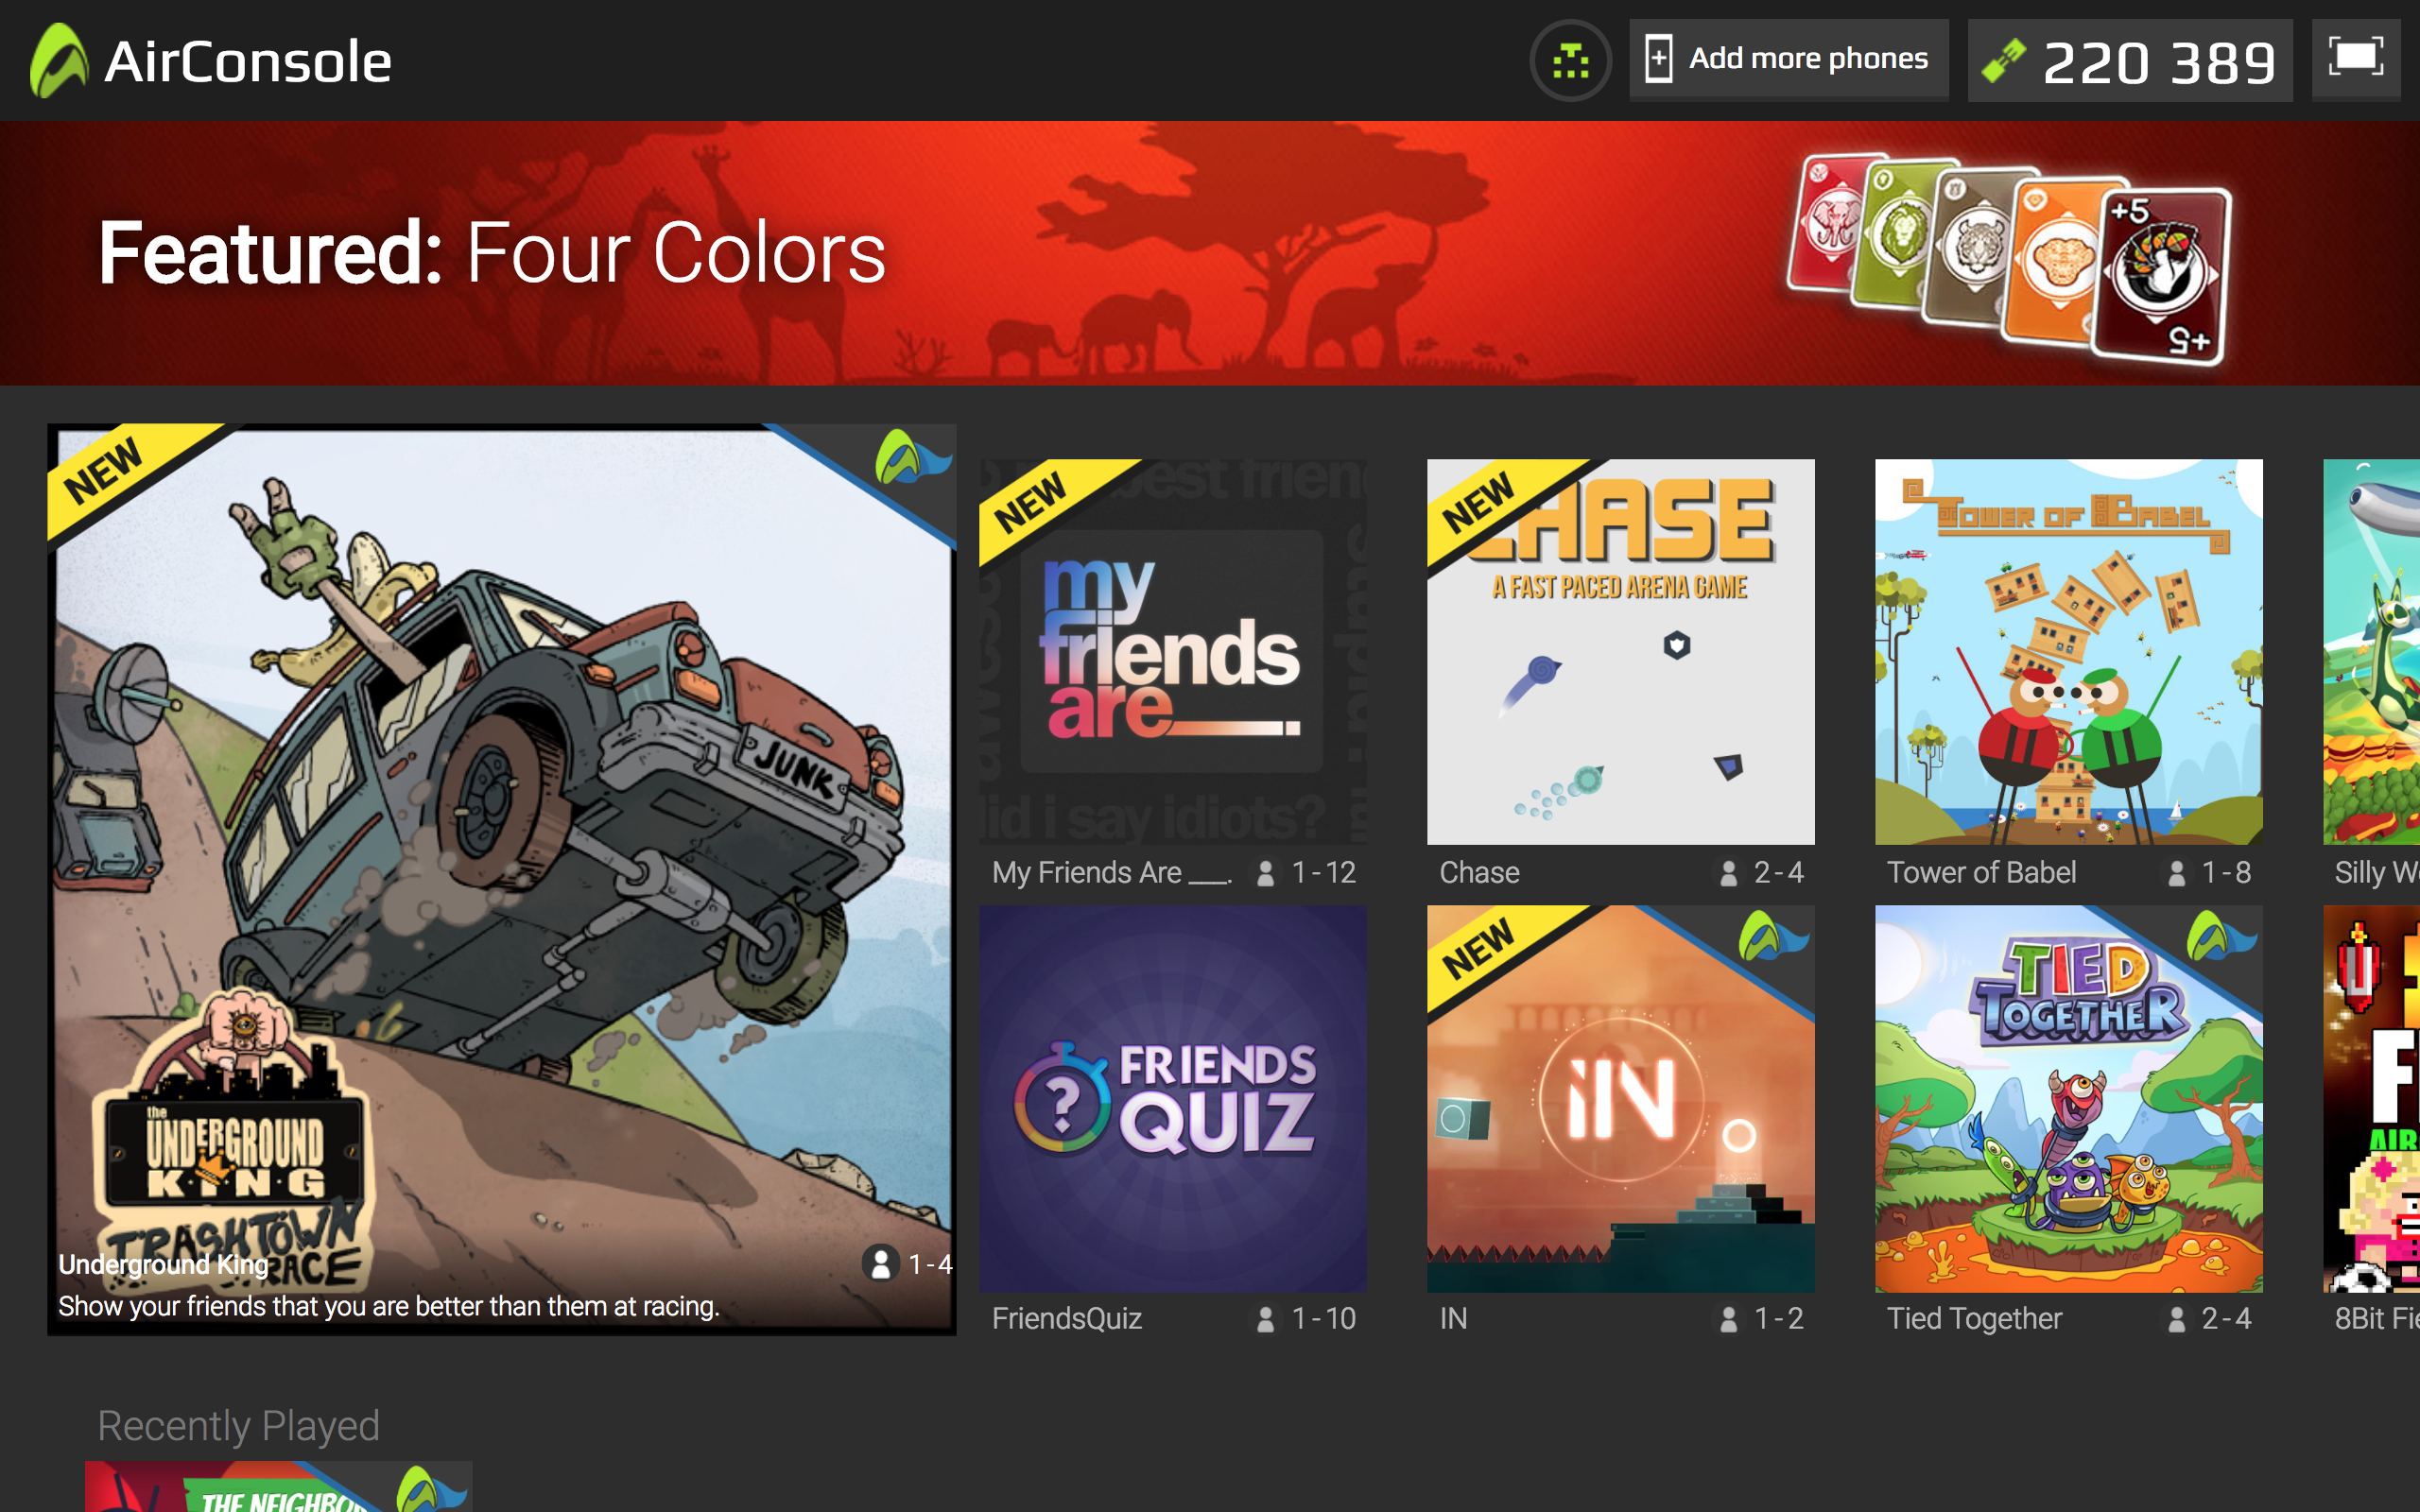
\includegraphics[scale=0.3]{Gambar/con3_play1}
	\caption{Halaman pada \textit{PC} yang menunjukan berbagai permainan yang dapat dipilih.}
	\label{fig:30_con3_play1}
\end{figure}
	
\end{enumerate}